%!TEX program = xelatex
\documentclass[UTF8]{ctexart}

\usepackage[utf8] {inputenc}
\usepackage {graphicx}
\usepackage {MnSymbol}
\usepackage {tikz}
\usepackage {media9}
\usetikzlibrary {arrows, shapes}
\usepackage {stmaryrd}
\usepackage {colortbl}
\usepackage {caption}
\usepackage {comment}
\usepackage {pdfpages}
\usepackage {listings}
\usepackage {color}
\usepackage {booktabs}
\usepackage {soul}
\usepackage[normalem] {ulem}

\usepackage {tcolorbox}
\usepackage {lipsum}
\usepackage {pgf}
\usepackage {etex}
\usepackage {tikz, pgfplots}

\tikzstyle {every picture} +  = [remember picture]
\everymath {\displaystyle}

\usepackage[square, numbers] {natbib} % \bibliographystyle {unsrtnat}

\hypersetup {
colorlinks = true, 
linkcolor = blue, 
filecolor = magenta, 
urlcolor = cyan, 
}

\mode<presentation> {

% The Beamer class comes with a number of default slide themes
% which change the colors and layouts of slides. Below this is a list
% of all the themes, uncomment each in turn to see what they look like.

%\usetheme{default}
%\usetheme{AnnArbor}
%\usetheme{Antibes}
%\usetheme{Bergen}
%\usetheme{Berkeley}
%\usetheme{Berlin}
%\usetheme{Boadilla}
%\usetheme{CambridgeUS}
%\usetheme{Copenhagen}
%\usetheme{Darmstadt}
%\usetheme{Dresden}
%\usetheme{Frankfurt}
%\usetheme{Goettingen}
%\usetheme{Hannover}
%\usetheme{Ilmenau}
%\usetheme{JuanLesPins}
%\usetheme{Luebeck}
%\usetheme{Madrid}
\usetheme{Malmoe}
%\usetheme{Marburg}
%\usetheme{Montpellier}
%\usetheme{PaloAlto}
%\usetheme{Pittsburgh}
%\usetheme{Rochester}
%\usetheme{Singapore}
%\usetheme{Szeged}
%\usetheme{Warsaw}

% As well as themes, the Beamer class has a number of color themes
% for any slide theme. Uncomment each of these in turn to see how it
% changes the colors of your current slide theme.

%\usecolortheme{albatross}
%\usecolortheme{beaver}
%\usecolortheme{beetle}
%\usecolortheme{crane}
%\usecolortheme{dolphin}
%\usecolortheme{dove}
%\usecolortheme{fly}
%\usecolortheme{lily}
%\usecolortheme{orchid}
%\usecolortheme{rose}
%\usecolortheme{seagull}
%\usecolortheme{seahorse}
\usecolortheme{whale}
%\usecolortheme{wolverine}

%\setbeamertemplate{footline} % To remove the footer line in all slides uncomment this line
% To replace the footer line in all slides with a simple slide count uncomment this line
\setbeamertemplate{footline}[page number]
% To remove the navigation symbols from the bottom of all slides uncomment this line
\setbeamertemplate{navigation symbols}{}
\usefonttheme {professionalfonts}
\useoutertheme {infolines}
\useinnertheme {circles}
}


\newtheorem *  {bem} {Bemerkung}

\usepackage {tikz}

\usepackage {listings}
\usepackage {color}

\definecolor {dkgreen} {rgb} {0, 0.6, 0}
\definecolor {gray} {rgb} {0.5, 0.5, 0.5}
\definecolor {mauve} {rgb} {0.58, 0, 0.82}

\lstset {frame = tb, 
language = Java, 
aboveskip = 2mm, 
belowskip = 12mm, 
showstringspaces = false, 
columns = flexible, 
basicstyle =  {\small\ttfamily}, 
numbers = none, 
numberstyle = \tiny\color {gray}, 
keywordstyle = \color {blue}, 
commentstyle = \color {dkgreen}, 
stringstyle = \color {mauve}, 
breaklines = true, 
breakatwhitespace = true, 
tabsize = 2
}
\lstdefinelanguage{code_example}{
  keywords={},
  keywordstyle=\color{orchid}\bfseries,
  keywords=[2]{for, reduce, doall},
  keywordstyle=[2]\color{blue1}\bfseries,
  keywords=[3]{load, store},
  keywordstyle=[3]\color{commentsColor}\bfseries,
  sensitive=false,
  comment=[l]{//},
  morecomment=[s]{/*}{*/},
  commentstyle=\color{byzantium}\ttfamily,
  stringstyle=\color{dkgreen},
  morestring=[b]',
  morestring=[b]",
  escapeinside={(:}{:)}
}

\definecolor{brown}{RGB}{166,42,42}
\definecolor{orchid}{RGB}{153,50,205}

\lstdefinelanguage{cute}{
  keywords={},
  keywordstyle=\color{orchid}\bfseries,
  keywords=[2]{typename, auto, for, int, using, decltype, uint128_t, half},
  keywordstyle=[2]\color{blue1}\bfseries,
  keywords=[3]{_1, _2, _4, _8,  _32},
  keywordstyle=[3]\color{maroon}\bfseries,
  keywords=[4]{make_tiled_copy},
  keywordstyle=[4]\color{dkgreen}\bfseries,
  sensitive=false,
  comment=[l]{//},
  morecomment=[s]{/*}{*/},
  commentstyle=\color{byzantium}\ttfamily,
  stringstyle=\color{dkgreen},
  morestring=[b]',
  morestring=[b]",
  escapeinside={(:}{:)}
}

\definecolor{sienna}{RGB}{160,82,45}
\lstdefinelanguage{fractaltensor-hello-world}{
  keywords={},
  otherkeywords={@, +, *, zeros, repeat},
  keywordstyle=\color{orchid}\bfseries,
  keywords=[2]{map, scan, fold, reduce},
  keywordstyle=[2]\color{red}\bfseries,
  keywords=[3]{xsss, xss, us, ws, bs},
  keywordstyle=[3]\color{dkgreen}\bfseries,
  keywords=[4]{ysss},
  keywordstyle=[4]\color{forestgreen}\bfseries,
  keywords=[5]{float32, FT},
  keywordstyle=[5]\color{sienna}\ttfamily\bfseries,
  keywords=[6]{zip},
  keywordstyle=[6]\color{blue}\ttfamily\bfseries,
  identifierstyle=\color{black},
  sensitive=false,
  comment=[l]{//},
  morecomment=[s]{/*}{*/},
  commentstyle=\color{byzantium}\ttfamily,
  stringstyle=\color{dkgreen},
  morestring=[b]',
  morestring=[b]",
  escapeinside={(:}{:)}
}

\renewcommand{\ttdefault}{pcr}
\lstdefinelanguage{cplus}{
  keywords={class, function, union, public, for, if, else, len, elif},
  keywordstyle=\color{forestgreen}\bfseries,
  keywords=[2]{TensorShape, NumberType, TensorType, FractalTensorType,
               ElemType, Collections, Number,
               TypeBase, FractalTensor, Tensor,
               float32, range, in, 
               int, void, bool, size_t, string, std,
               unique_ptr, vector, int64_t},
  keywordstyle=[2]\color{blue}\bfseries,
  keywords=[3]{const},
  keywordstyle=[3]\color{tomato}\bfseries,
  keywords=[4]{xss, yss, ysss, w, ws, L, N, D},
  keywordstyle=[4]\color{dkgreen}\bfseries,
  keywords=[5]{zeros, @, +},
  keywordstyle=[5]\color{orchid}\bfseries,
  identifierstyle=\color{black},
  sensitive=false,
  comment=[l]{//},
  morecomment=[s]{/*}{*/},
  commentstyle=\color{grey}\ttfamily,
  stringstyle=\color{dkgreen},
  morestring=[b]',
  morestring=[b]",
  escapeinside={(:}{:)}
}

\title{RNNs and scan}

\begin{document}

\tableofcontents
\thispagestyle{empty}
\newpage
\setcounter{page}{1}

\bibliographystyle{plain}

\noindent
\linespread{1.2}
\selectfont
\setlength{\topskip}{0ex}
\setlength{\parskip}{1ex}
\setlength{\lineskip}{1em}

\section{Transformer和线性RNN}
\noindent \textbf{Notations}: $\mathbf{X}$表示矩阵,$\vec{x}$表示列向量。

\begin{figure}[h]
    \centering
    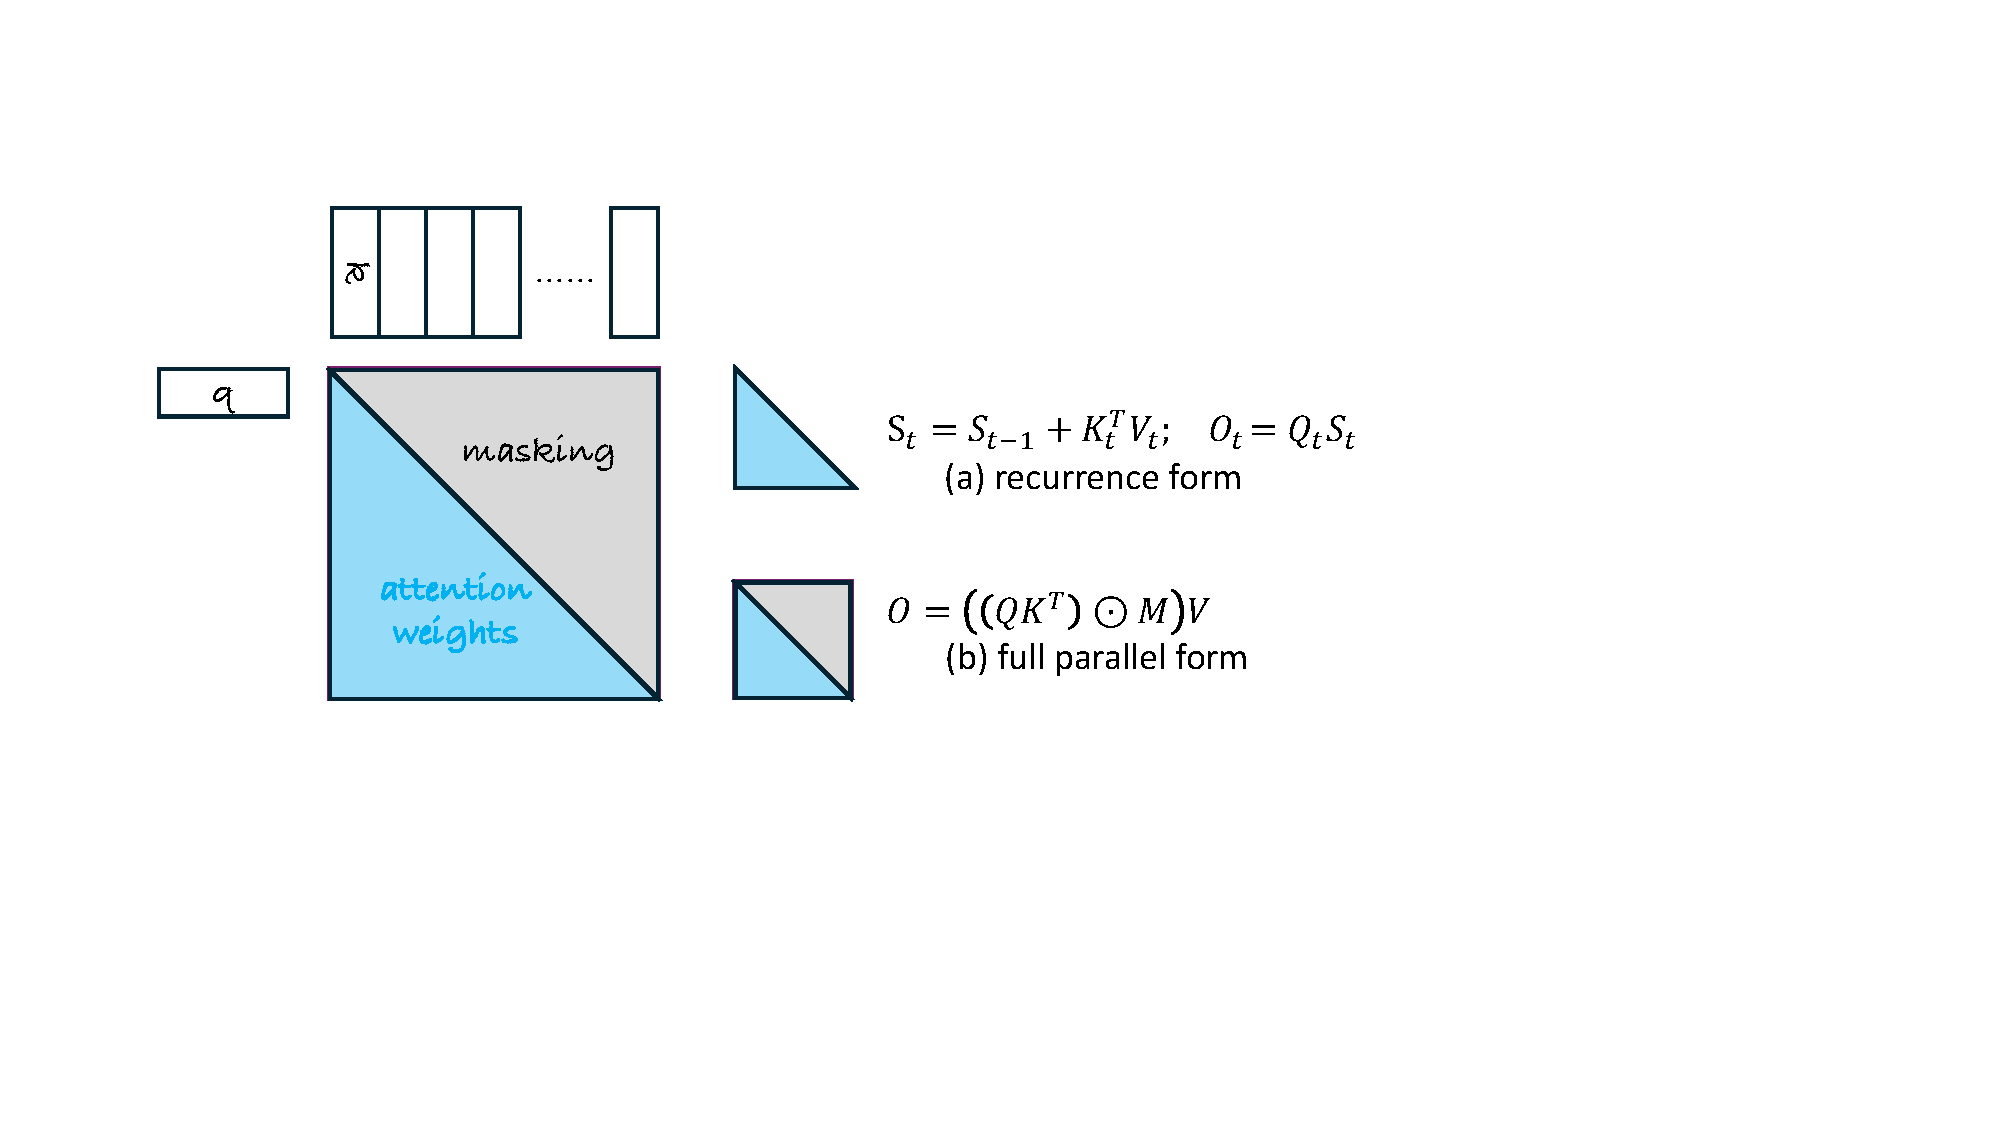
\includegraphics[width=0.6\textwidth]{figures/attention-train.pdf}
    \caption{Transformer的两种计算模式:recurrent form和full parallel form}\label{fig:attention-train}
\end{figure}

训练时我们可以一次性看到全序列,如果token之间不存在数据流依赖,就可以让query token
\footnote{\textbf{\textcolor{red}{这是我们要研究的第一种计算模式。}}}{\colorbox{thistle}{全并行计算}}。

如图\ref{fig:attention-train}所示,上三角部分是冗余计算,通过masking机制消除。
Attention的全并行方式是直接将for循环在空间上全展开。
空间全展开情况下上图上三角部分是冗余计算,需要后续靠点乘一个masking矩阵消除这部分多余计算。

\subsection{Linear Attention\cite{linear-attention-kexue}}

\begin{equation}
O = \text{Attention}(\mathbf{Q},\mathbf{K},\mathbf{V}) = \text{softmax}(\mathbf{Q}\mathbf{K}^T)\mathbf{V} \label{eq:attn1}
\end{equation}

上述公式是多头注意力机制中一个头如何计算的线性代数公式。
其中$\mathbf{Q} \in \mathbb{R}^{L \times d}$,$\mathbf{K}^T \in \mathbb{R}^{d \times L}$,$\mathbf{V} \in \mathbb{R}^{L \times d}$。

目前Transformer模型广泛被用来处理超长序列。假设$E$是隐藏层的维度(一般$E = 512,1024,2048$,在这样的量级)。如果应用了多头注意力机制,会对隐藏层分头$d = \frac{E}{\text{num\_head}}$。
于是$L\gg d$,$\mathbf{P} = \mathbf{Q}\mathbf{K}^T \in \mathbb{R}^{L \times L}$这一步会得到一个非常大的$L^2$大小的中间结果。

仔细分析会发现\textbf{\textcolor{red}{影响attention进一步扩展的是softmax}}。

矩阵乘满足结合律,如果没有softmax,我们可以先计算$\mathbf{S} = \mathbf{K}^T \mathbf{V}$: $[d \times L] [L \times d] = [d \times d]$,得到中间结果大小为$d\times d$,再计算$\mathbf{O} = \mathbf{Q}\mathbf{S}$。由于$d \ll L$,这样的计算过程也会近似地与序列长度呈线性复杂度。

观察attention的sequential计算公式(\textcolor{maroon}{换一种语言来说这里的“sequential计算公式”,也就是把"matrixfied"的线性代数公式展开写成$\sum$求和}):
$$\text{Attention}(\vec{q}_t, \mathbf{K}, \mathbf{V}) = \frac{\sum_{i=0}^{t}\exp \left(\vec{q}_t \vec{k}_i^T\right)\vec{v}_i}{\sum_{i=0}^{t}\exp \left( \vec{q}_t \vec{k}_i^T \right)}$$

我们可以把attention理解为以$\exp \left( \vec{q}_t \vec{k}^T_i \right)$为权值,对$\vec{v}_i$进行加权再求和。于是可以提出一个泛化版的attention:

$$\text{Attention}\left( \vec{q}_i, \mathbf{K}, \mathbf{V} \right) = \frac{\sum_{t=0}^{L}\text{sim} \left(\vec{q}_i, \vec{k}_t \right) \vec{v}_j}{\sum_{t=0}^{L}\text{sim} \left( \vec{q}_i,\vec{k}_t \right)}$$

为了\textcolor{dkgreen}{保持attention的输出结果是一个分布这一关键特性,\textbf{我们要求$\text{sim}(q_t,k_i)\ge 0$}}\footnote{每个分量$\ge 0$是分布的一个最低要求,softmax会得到一个严格的概率分布,求和为0}{。}
基于以上分析,可扩展attention转换为如何设计$\text{sim}\left( \vec{q}_i, \vec{k}_j \right)$。

寻找一个总是大于0的相似度函数可以被转换为许多不同的解决思路,\cite{katharopoulos2020transformers}用了一种简单的思路,给$\vec{q}_t$和$\vec{k}_i$加上限制了值域的激活函数,然后使用内积作为相似性度量。这种方法被解释为“kernel method"。于是我们有如下公式:

$$\vec{o}_t = \frac{\sum_{i=0}^{t}\phi \left( \vec{q}_t \right)\phi \left(\vec{k}_i \right)^T \vec{v}_i}{\sum_{i=0}^{t}\phi \left(\vec{q}_t \right) \phi \left( \vec{k}_i\right)^T} = \frac{\phi \left( \vec{q}_t \right) \sum_{i=0}^{t}\phi \left( \vec{k}_i \right)^T \vec{v}_i}{\phi \left(\vec{q}_t\right) \sum_{i=0}^{t} \phi \left(\vec{k}_i \right)^T}$$

$\mathbf{S}_t \triangleq \sum_{i=0}^{t} \phi \left( \vec{k}_i \right)^T\vec{v}_i$,$\vec{z}_t \triangleq \sum_{i=0}^{t} \phi \left(\vec{k}_i\right)^T$,于是有:

\begin{align}
\mathbf{S}_t &= \mathbf{S}_{t-1} + \phi \left( \vec{k}_t \right)^T\vec{v}_t \nonumber\\
\vec{z}_t &= \vec{z}_{t-1} + \phi \left( \vec{k}_t \right)^T \nonumber \\
\mathbf{O}_t &= \frac{\phi \left( \vec{q}_t \right) \mathbf{S}_t}{\phi \left( \vec{q}_t \right) \vec{z}_t} \label{eq:linear-attn1}
\end{align}

式\eqref{eq:linear-attn1}就是一个泛化版attention框架,不同的工作对$\phi$进行了探索。\textcolor{red}{(1)认为$\phi$取indentity function in practice也够用。(2)有些工作claim 归一化因子$\vec{z}_t$会引起不稳定性,建议可以扔掉$\vec{z}_t$,在输出增加归一化计算},
于是会得到一个如下形式的未归一化的linear attention Transformer:

\begin{align}
\mathbf{S}_t &= \mathbf{S}_{t-1} + \vec{k}_t^T\vec{v}_t \label{eq:linear-attn2}\\
\vec{o}_t &= \vec{q}_t\mathbf{S}_t \nonumber
\end{align}

\textcolor{red}{linear-attention}当作\footnote{\textcolor{red}{这是我们要研究的第二种计算模式。}}{\colorbox{thistle}{RNN式的递归式来}}计算时(图\ref{fig:attention-train}(a)),模型的时间和空间复杂度是序列长度的线性关系,能够节约FLOPS,但是会引入串行性。

如果我们把attention按照下式当作一个矩阵乘来计算(图\ref{fig:attention-train}(b)),模型的时间和空间复杂度是序列长度的平方关系,优点是可以全并行计算。

$$\mathbf{O} = \left( \left(\mathbf{Q}\mathbf{K}^T\right) \odot \textcolor{red}{\mathbf{M}} \right)\mathbf{V}$$

上式$\textcolor{red}{\textbf{M}}$会破坏矩阵乘的结合性,导致如果我们想通过并行方式(时间维度的计算在空间维度全展开),
依然必须先算$\mathbf{Q}\mathbf{K}^T$,再与$\mathbf{V}$相乘,
还是会引起需要存储$L^2$大小的中间结果。

为了让这类模型高效训练,一个折中方案是\footnote{\textcolor{red}{这是我们要研究的第三种计算模式。}}{\colorbox{thistle}{Chunk-wise Block-parallel}} attention。

\begin{align*}
\mathbf{O}_{i+1} &= \mathbf{Q}_{i+1}\mathbf{S}_{i} + \left( \left(\mathbf{Q}_{i+1}\mathbf{K}_{i+1}^T\right) \odot \textcolor{red}{\mathbf{M}} \right)\mathbf{V}_{i+1} \in \mathbb{R} ^{C\times d} \\
\mathbf{S}_0 &= \mathbf{0}
\end{align*}

% \begin{tcolorbox}[colbacktitle=grey!10!white,colback=yellow!3,title={\textbf{\textcolor{grey}{My Take-aways}}}]
% 一个DNN算法是一组任意复杂的线性代数,由于算律满足一定条件\textcolor{red}{(不确定是否能够准确地定义出必要条件?)}会存在两种等价形式:\textit{\textcolor{brown}{空间展开的全并行形式}} vs. \textit{\textcolor{brown}{时间展开的串行方式}},这两种等价形式对系统来说,可能会是一个潜在的调度/决策空间。
% \end{tcolorbox}

\subsection{Linear Attention with Decay}

\colorbox{snow}{\eqref{eq:linear-attn2}显示地表明:\textcolor{red}{\textbf{带线性attention的Transformer,就是一个隐状态是矩阵的RNN}}}。
有许多研究指出,为RNN的state引入decay(衰减)机制,类似于遗忘门的能力,能够有效的改善学习效果。于是引入衰减因子\textcolor{red}{$\gamma$},\eqref{eq:linear-attn2}式改写成如下形式:

\begin{align}
\mathbf{S}_t &= \textcolor{red}{\gamma} \mathbf{S}_{t-1} + \mathbf{K}_t^{T}\mathbf{V}_t
\end{align}

对应的并行形式:

\begin{align*}
\mathbf{O} &= \left( \mathbf{Q}\mathbf{K}^T \odot \mathbf{D}\right)\mathbf{V},
&\mathbf{D} &= \left\{
\begin{aligned}
  &\gamma^{n-m}, &n \ge m \\
  &0, &n < m
\end{aligned}
\right.
\end{align*}

\subsection{典型代表}

\subsubsection{RetNet\cite{sun2023retentive}}

RNN模型相关研究表明:遗忘门对改善学习效果有着重要作用。

在DNN模型学习效果方面,RetNet的一个设计要素是:在recurrent计算对状态的更新过程中,
引入一个显示的衰减(decay term)能够极大的改善学习效果,一些情况下甚至可以超过标准的softmax Transformer。

\begin{displayquote}
adding a global decay term to the additive RNN update rule greatly improves performance, sometimes outperforming standard Transformers with softmax attention when trained at scale.\cite{yang2023gated}
\end{displayquote}

\subsubsection{GAU\cite{hua2022transformer}}

\subsubsection{GLA\cite{yang2023gated}}


\section{SSM(state-space model)}
SSM是一个非常广泛的概念,可以认为带有隐状态的循序计算都是SSM模型。
他的思想和和RNN,CNN,Attention这样的神经网络完全不同,背后的想法是让把序列看做是对一个动态系统的离散采样,SSM模型通过微分方程组来建模动态系统状态随时间的变化。

\subsection{一个朴素的直觉解释}

我们首先通过一个全标量计算模型,建立起对state-space model的直觉理解。

\begin{tcolorbox}[colbacktitle=grey!10!white,colback=yellow!3,title={\textbf{\textcolor{grey}{用微分方程组建模动态系统,一个极简例子}}}]
这个\href{https://www.youtube.com/watch?v=8Q_tqwpTpVU}{video}(对应的\href{https://github.com/hkproj/mamba-notes/tree/main}{slides})里speaker举了一个具体的例子来解释用微分方程组建模一个动态系统。
假设我们有一群兔子,每只小兔子在$t$时刻会生$\lambda$只小兔子,$\lambda$是一个固定的常数。
令$b(t)$表示$t$时刻兔子种群一共有多少只兔子,$\frac{db}{dt}$表示$t$时刻兔子种群数目变化的速率,于是有:

$$\frac{db}{dt}=\lambda b(t)$$

已知$t=0$时刻种群有5只兔子,即:$b(t)=5$。我们希望求解出$b(t)$的方程使得对任意$t$,上式都成立,来告诉我们任意时刻,例如$t=100$,种群有多少只兔子。
\end{tcolorbox}

连续时间系统线性SSM模型(continuous-time linear/latent state-space model)将输入信号$x(t)$通过一个隐状态$h(t)$映射到输出信号$y(t)$。

\begin{align}
    h'(t) &= \mathbf{A}h(t) + \mathbf{B}x(t) \label{eq:ssm1}\\
    y(t) &=\mathbf{C}h(t) + \mathbf{D}x(t) \label{eq:ssm2}
\end{align}

\eqref{eq:ssm1}和\eqref{eq:ssm2}已经规定了微分方程组的具体形式,参数化为$\mathbf{A}$,$\mathbf{B}$,$\mathbf{C}$和$\mathbf{D}$。
这样一组微分方程可以用来建模一个动态系统其状态随时间的改变。
求解目标是求解出以上微分方程的具体形式,使得给定系统在0时刻的初始状态,能够计算得到这个动态系统在任意时刻的状态。

为了求解上面这个微分方程组,我们需要找到$h(t)$的具体形式令\eqref{eq:ssm1}等号左右两边相当。
通常情况下找到$h(t)$的解析解是困难的。因此,我们降低要求,\textcolor{tomato}{考虑找到$h(0)$,$h(1)$,$h(2)$,etc.这样一个离散化的序列,用来逼近我们要研究的动态系其状态如何随时间改变}。
因此,我们将寻找$h(t)$转化为对时间进行离散化采样,$k$是采样编号,寻找一个离散化序列$h(t_k) = h(k \triangle)$使以上微分方程系统近似地成立。其中,$\triangle$是step size。

根据导数的定义,我们有:$h'(t) = \lim_{\triangle \rightarrow 0}\frac{h(t+\triangle)-h(t)}{\triangle}$,当step size$\triangle$足够小的时候,我们可以省略极限符号:
$$h(t + \triangle) \approxeq \triangle h'(t) + h(t)$$

将\eqref{eq:ssm1}带入,可得:

\begin{align}
    h(t+\triangle) & \approxeq \triangle \left( \mathbf{A}h(t) + \mathbf{B}x(t)\right) + h(t) \nonumber \\
    &=\triangle \mathbf{A} h(t) + \triangle \mathbf{B}x(t)+h(t) \nonumber \\
    &=\left(\mathbf{I} +\triangle A\right)h(t) + \triangle \mathbf{B} x(t) \nonumber \\
    &\triangleq \bar{\mathbf{A}}h(t) + \bar{\mathbf{B}}x(t) \label{eq:ssm3}
\end{align}

式\eqref{eq:ssm3}是SSM的离散化形式。

\subsection{SSM}

机器学习任务中隐状态均为高维,从上一节的标量形式进一步推广到高维可以参看s4\cite{gu2021efficiently}的论文,这里我们仅关注需要知道的最基本事实。
一个SSM模型的求解需要经过离散化(Zero-Order-Hold(ZOH)或者Bilinear方法),
离散化形式的SSM由以下两个公式表示,其中$\vec{x}$是状态,$\vec{u}$是输入信号,$\vec{y}$是输出信号,

\begin{align}
  \vec{h}_k &= \bar{\mathbf{A}}\vec{x}_{k-1} + \bar{\mathbf{B}}\vec{u}_k \label{eq:ssm4}\\
  \vec{y}_k &= \bar{\mathbf{C}}\vec{x}_k + \bar{\mathbf{D}}\vec{u}_k 
\end{align}

离散化方法会进一步给出$\bar{\mathbf{A}}$,$\bar{\mathbf{B}}$和$\bar{\mathbf{C}}$矩阵的进一步形式。

\textcolor{red}{为了让离散化操作能快速地完成计算,会对矩阵$\mathbf{A}$的形式有所约束,例如为了让矩阵的幂运算快速实现,要求$\mathbf{A}$是一个对角矩阵}。

在预测时候和RNN等价,SSM参数化形式为一组用微分方程组描述的,带隐状态的连续时间系统。通过恰当的离散化方法,能够被转换成CNN或RNN计算。

预测时SSM和RNN计算等价,但是SSM这一类模型的设计来源于不同的理论框架,在训练时有可能带来不同的特性。

\subsection{SSM和RNN的不同之处}

DeepMind的LRU\cite{orvieto2023resurrecting}也讨论了SSM和RNN的不同。

\begin{enumerate}
\item SSM模型离散化之后根据定义\textcolor{red}{在时间维度上是线性的}。也就是说,SSM by definition就是一个linear RNN,在训练的时候适用于以parallel scan模型并行地进行计算;
\item 尽管式\eqref{eq:ssm4}是一个RNN,但是其中$\mathbf{A}$和$\mathbf{B}$有更强的参数化要求。例如,ZOH离散化方法会给出:$\bar{\mathbf{A}}=\exp\left(\triangle \mathbf{A}\right)$,
$\bar{\mathbf{B}}=\left(\bar{\mathbf{A}} -\mathbf{I}\right)\mathbf{A}^{-1} \mathbf{B}$,$\bar{\mathbf{C}}=\mathbf{C}$,
$\bar{\mathbf{D}}=\mathbf{D}$。
\item SSM的初始化非常特殊。recurrent形式的全展开涉及到矩阵的幂运算。为了高效计算矩阵的幂,会要求$\mathbf{A}$是对角矩阵。然而无法总是在实数域将$\mathbf{A}$对角化,但是几乎所有矩阵都能在复数域上对角化,于是SSM将运算放在了复数域,
\footnote{最新的研究通过新的技术放松对这一点的要求}{SSM需要特殊设计的初始化计算}。
\end{enumerate}

\subsection{典型代表}

\subsubsection{S4(\textcolor{blue}{S}tructured \textcolor{blue}{S}tate \textcolor{blue}{S}pace \textcolor{blue}{S}equence models)\cite{gu2021efficiently}}

S4的第一个$S$代表了 "structured"。具体是指:为了SSM能够高效地并行训练,会对矩阵$A$的结构带来一定的约束,目前使用最多的一种约束是要求$A$是一个对角矩阵。

\subsubsection{S5\cite{smith2022simplified}}

\newpage
\subsubsection{Mamba(S6)\cite{gu2023mamba}}

受Transformer整体架构的影响,目前sequence processing模型都是通过反复堆叠一个同构的sequence processing block构成。
这样一个sequence processing block一般由归一化层, token mixer,residual connection三个设计要素构成。
mamba中的norm都用RMSnorm。

\begin{figure}[h]
  \centering
  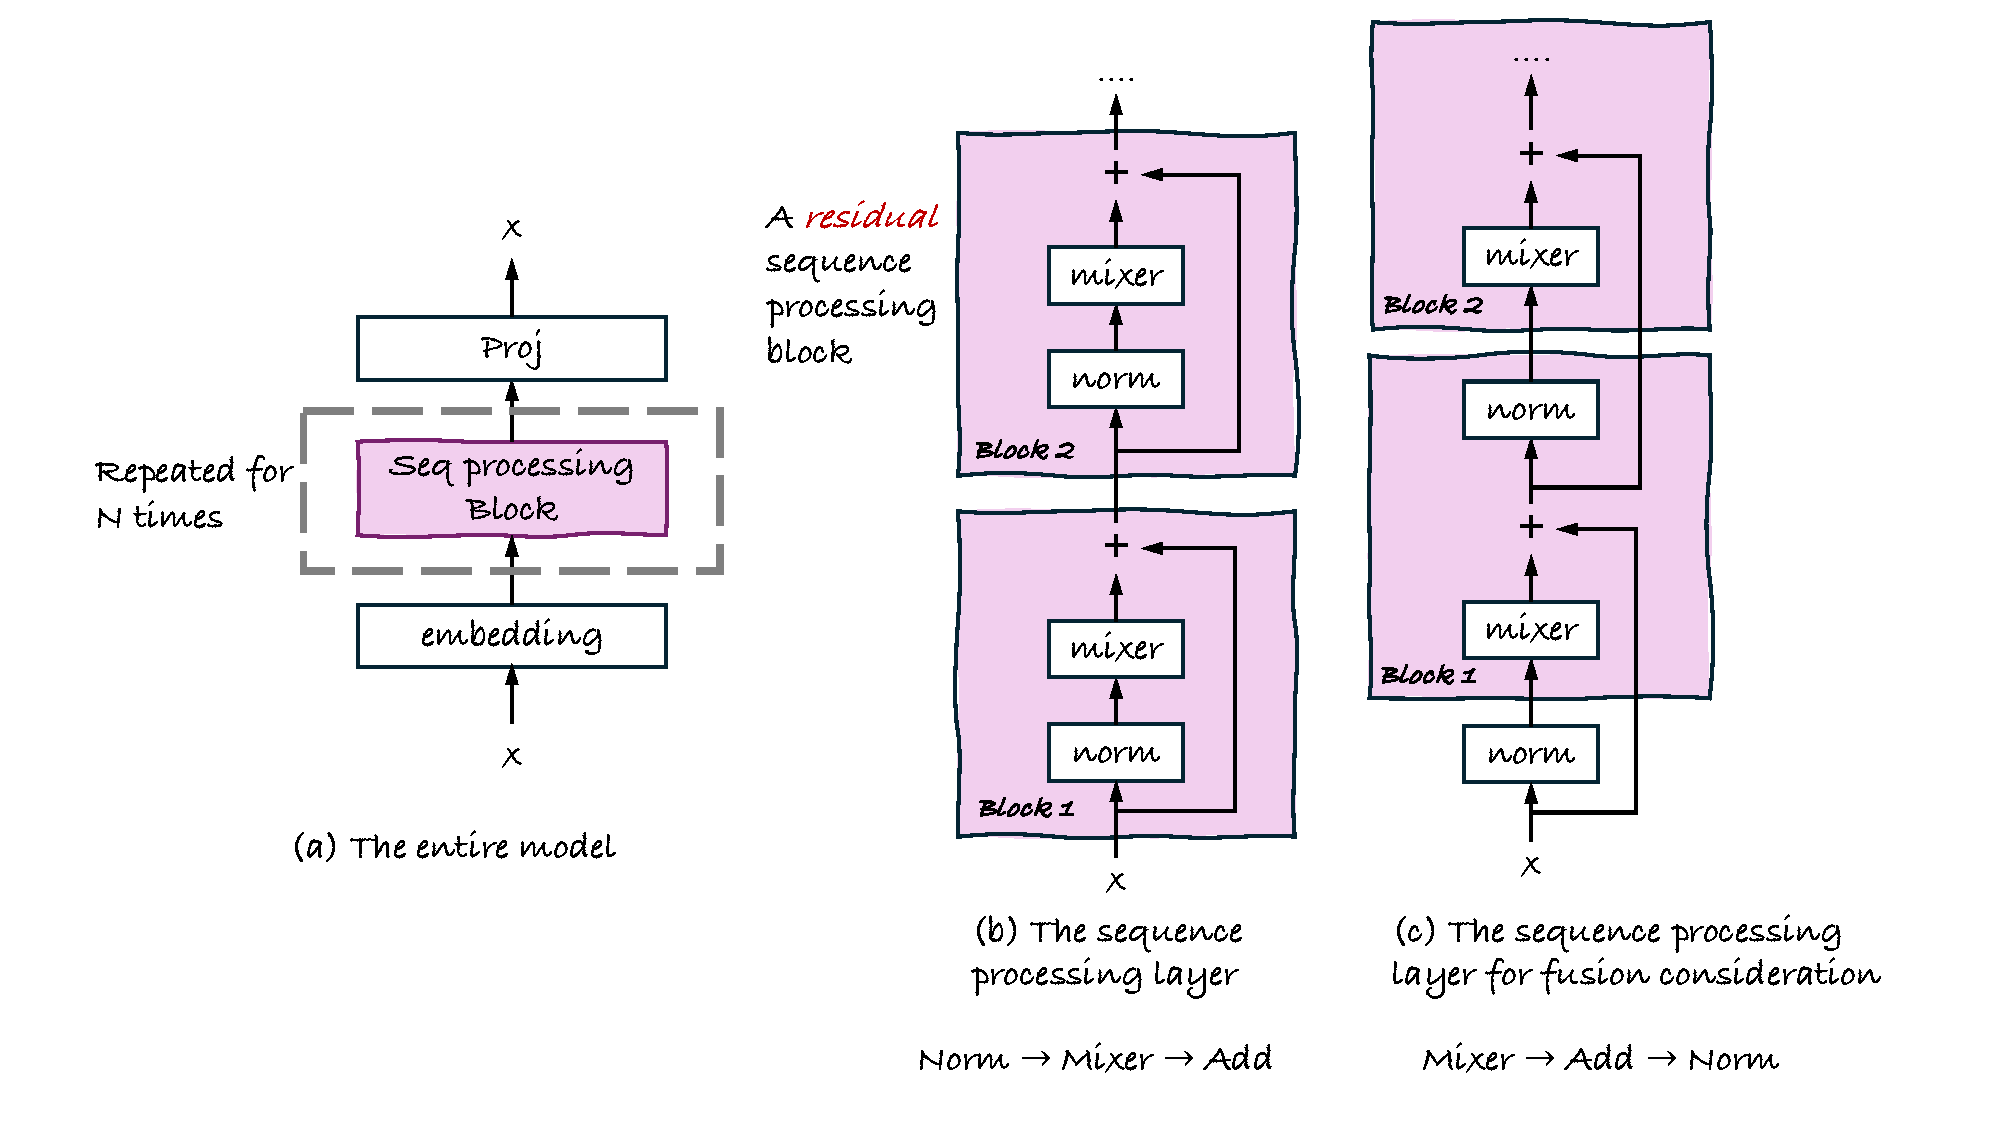
\includegraphics[width=0.85\textwidth]{figures/mamba-model.pdf}
  \caption{mamba模型的整体结构}\label{fig:mamba-model}
\end{figure}

图\ref{fig:mamba-model}(b)的Norm $\rightarrow$ Mixer $\rightarrow$ Add串block的方式更符合设计直觉。
图\ref{fig:mamba-model}(a)的Mixer$\rightarrow$ Add $\rightarrow$ Norm串block的方式更容易在现有PyTorch接口下将Add和Norm进行fuse。

\begin{figure}[h]
  \centering
  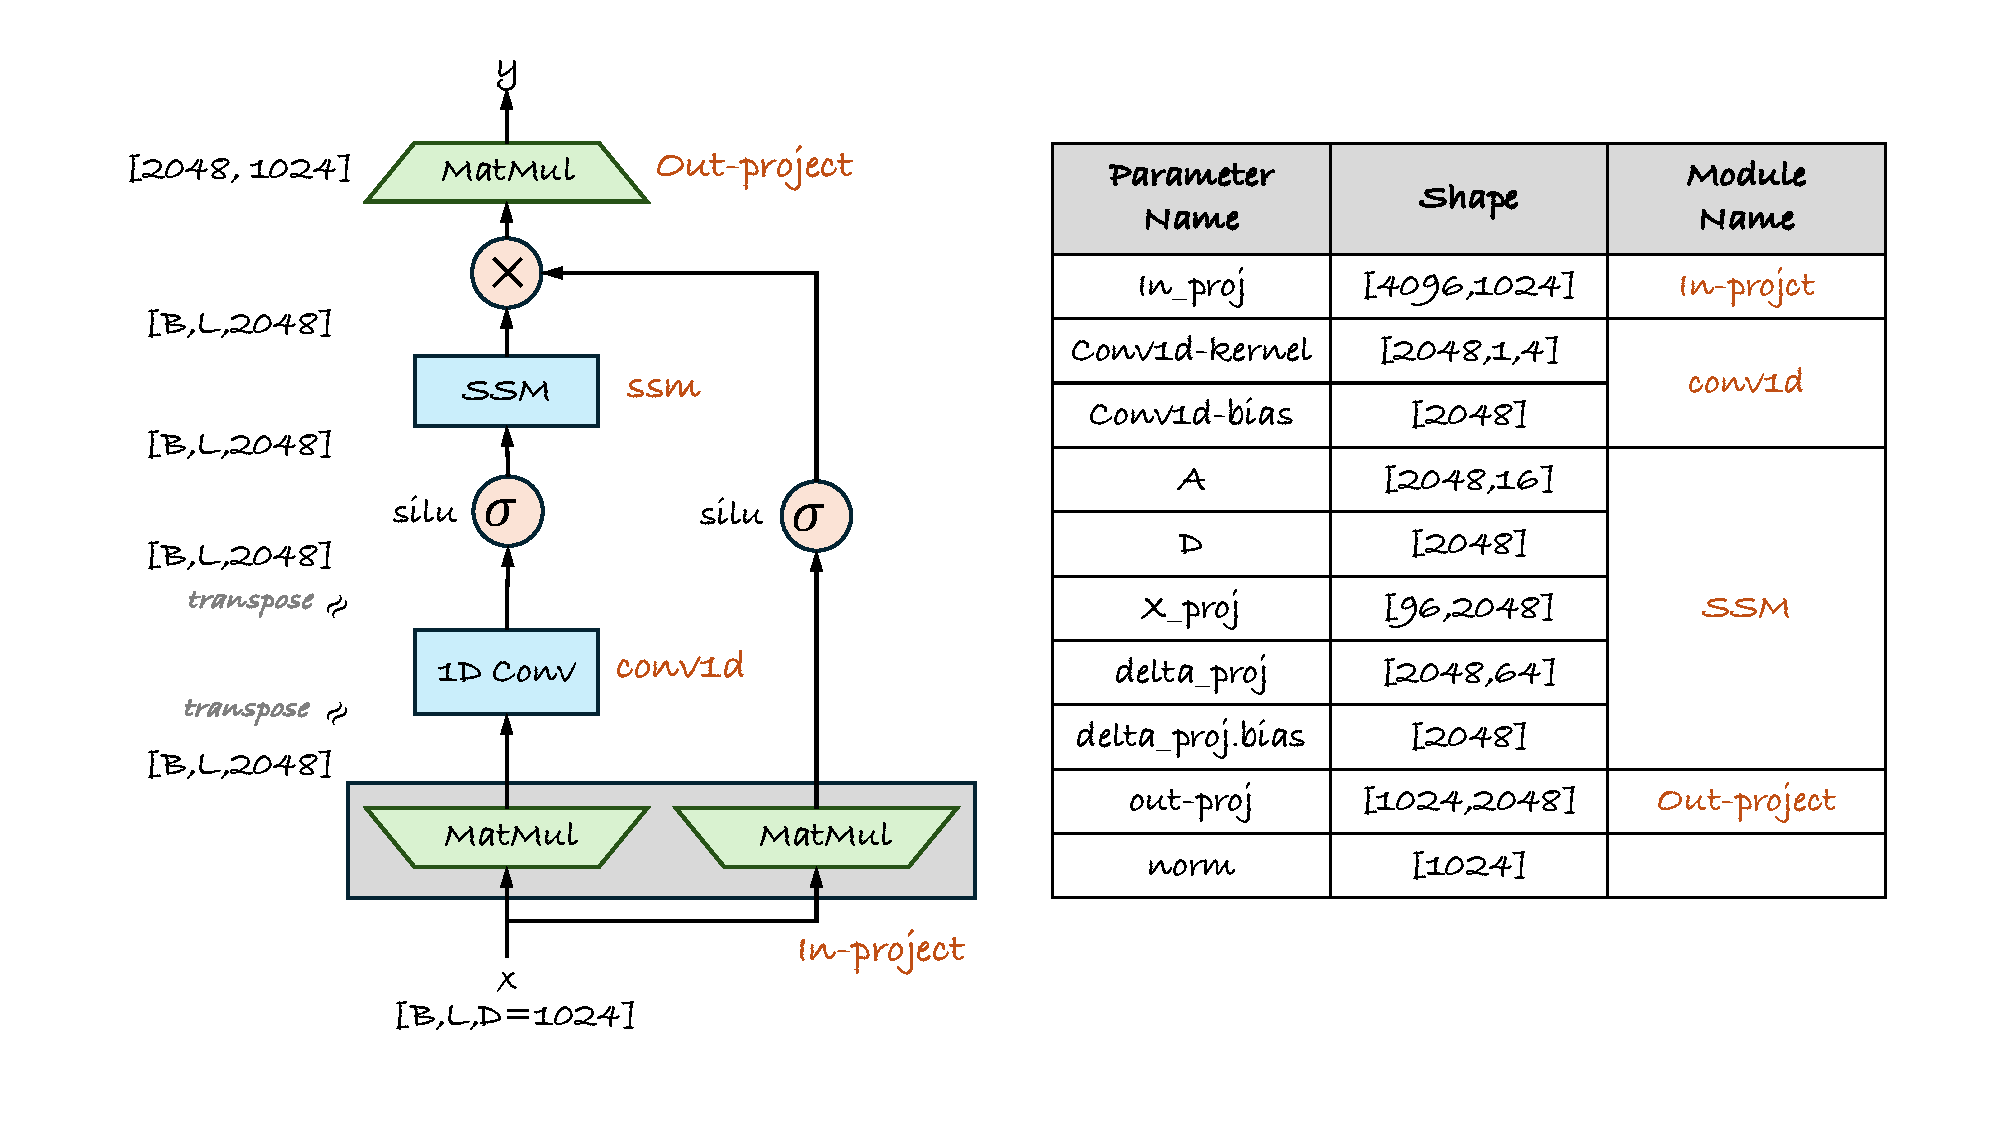
\includegraphics[width=0.9\textwidth]{figures/mamba-mixer.pdf}
  \caption{mamba block作为图\ref{fig:mamba-model}中mixer的细节及可学习参数}\label{fig:mamba-mixer}
\end{figure}

Mamba block是图\ref{fig:mamba-model}中mixer。
Mamba-370m模型里面mamba block堆叠$48$次,输入序列$X$的形状$[B,L,D]$,$D=1024$。

图\ref{fig:mamba-mixer}中SSM部分计算公式如下,其中$u(t)$是整个sequence batch,形状为$[B,L,2048]$,$x(t)$是SSM内部的状态:

\begin{equation}
y(t) = \text{SSM}(u(t)) \label{eq:ssm-0}
\end{equation}

\begin{figure}[h]
  \centering
  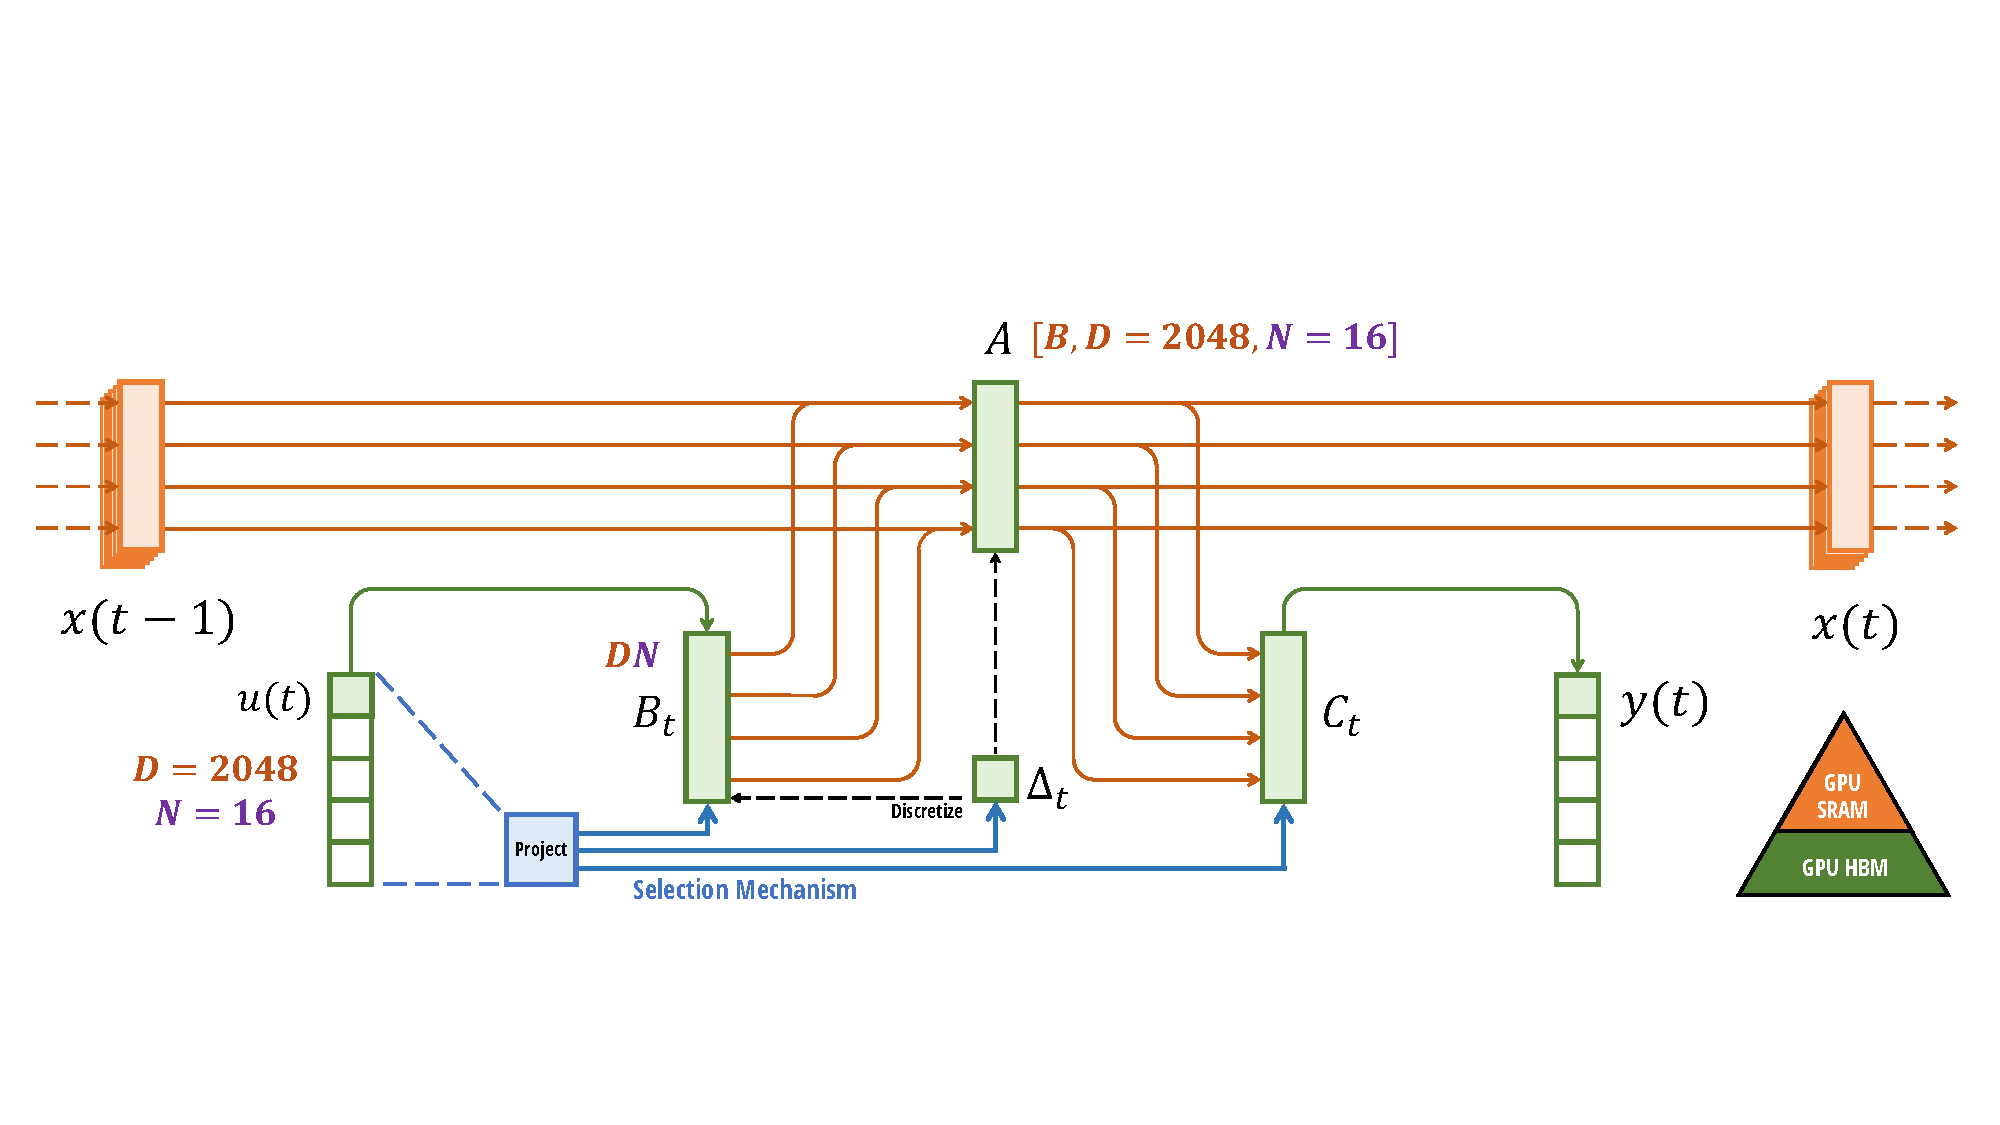
\includegraphics[width=0.9\textwidth]{figures/mamba-ssm.pdf}
  \caption{图\ref{fig:mamba-mixer}中SSM模块的细节}\label{fig:mamba-ssm}
\end{figure}

SSM内部带有隐状态$x(t)$,式\eqref{eq:ssm-0}通过隐状态$x(t)$把输入$u(t)$映射到$y(t)$。
一个离散化之后的SSM模型其可学习为:
\textcolor{red}{$\triangle$,$\mathbf{A}$,$\mathbf{B}$,$\mathbf{C}$,
$\mathbf{D}$}。
mamba中,$\mathbf{A}$和$\mathbf{D}$不依赖于输入;
$\mathbf{\triangle}$,$\mathbf{B}$和$\mathbf{C}$依赖于输入。

Listing \ref{ssm-code}中红色高亮的变量直接对应图\ref{fig:mamba-mixer}中右表中的可学习参数。

\begin{lstlisting}[language=cplus, caption={ssm in mamba},label={parallel-scan-mamba}, label={ssm-code}]
function SSM((:$u_{[B, L, 2048]}$:))(:$\rightarrow y(t)_{[B,L,2048]}$:)
  (:$v_0 = u(t)\ @ \ \textcolor{red}{\text{x\_proj}}^T$:)  // (:\textcolor{grey}{$[B,L,2048]@[2048,96]\rightarrow [B,L,96]$}:)
  (:$v_1, \mathbf{B}, \mathbf{C} = \text{split}(v_0)$:)  // (:\textcolor{grey}{$[B,L,64], [B,L,16], [B,L,16]$}:)
  (:$\triangle = \text{softplus}(v_1@\textcolor{red}{\text{delta\_proj}}^T + \textcolor{red}{\text{delta\_proj.bias}})$:) // (:\textcolor{grey}{$[B,L,64]@[2048,64]+[2048]\rightarrow [B,L,2048]$}:)
  (:$\bar{\mathbf{A}}=\exp\left(\triangle \textcolor{red}{\mathbf{A}}\right)$:)  // (:\textcolor{grey}{$[B,L,2048]@[2048,16]\rightarrow [B,L,2048,16]$}:)
  (:$\bar{\mathbf{V}}=\triangle\mathbf{B}u(t)$:) // (:\textcolor{grey}{$[B,L,2048]@[B,L,16]@[B,L,2048]\rightarrow [B,L,2048,16]$}:)

  // 9~12行是mamba代码中的selective_scan kernel
  (:$x(t)$:) = zeros((:$[B,2048,16]$:))  // scan的状态
  for (:$i$:) in (:$[0, L)$:):  // 把这个for循环实现成parallel scan
    (:$x(t) = \bar{\mathbf{A}}[:,i] * x(t) +\bar{\mathbf{V}}[:,i]$:)  // (:\textcolor{grey}{$[B, 2048, 16]$}:)
    (:$y(t)[:,i] = x(t) @ C[:,i]$:)  // bmm, (:\textcolor{grey}{$[B, 2048, 16]@[B,16]\rightarrow [B, 2048]$}:)
  (:$y(t) = y(t) + \textcolor{red}{\mathbf{D}}*u(t)$:)  // (:\textcolor{grey}{$[B, L, 2048]$}:)
\end{lstlisting}

% 其中$u(t)$的大小$[B, L, 2048]$, $A$大小$[2048,16]$,$D = 2048$,$A$和$D$是输入无关的,$\triangle$,$B$,$C$是input-dependent的(selective的)。

% \begin{enumerate}
% \item $v_0 = u(t) @ \textcolor{red}{W_1}$,$u(t)$是整个序列
% \item $v_1$, $B$, $C$ = $\text{split}(v_0)$,$v_1$用来计算$\triangle$,可以看到是输入相关的
% \item $\triangle = \text{softplus}(v_1 @ \textcolor{red}{W_2})$,这里$W_2$的大小是$[64,2048]$
% \item $y = \text{selective\_scan}(u(t), \triangle, A, B, C, D)$
% \end{enumerate}

% $W_1$的大小$[2048, 96]$,
% 这里的$96$是怎么来的呢?$96 = 64 + 16 * 2$。$64$是$\triangle$维度的大小,16是$B$和$C$的维度大小。
% 然后这个映射会被切分成$\triangle$,$B$和$C$

% $$y = \text{selective\_scan}(u, \triangle, \mathbf{A}, \mathbf{B}, \mathbf{C}, \mathbf{D})$$

% 上式中各个输入数据的大小:$u:[B, L, 2048]$,$\triangle:[B, L, 2048]$,$A:[2048,16]$,$B:[B, L, 16]$,$C:[B, L, 16]$,$D:[2048]$。

Listing \ref{ssm-code} 中5至13行对应了离散化SSM的两组公式:

\begin{align}
\bar{\mathbf{A}} &= \exp(\triangle \mathbf{A}) & [B, L, 2048, 16] \label{eq:mamba1}\\
\bar{\mathbf{V}} &= \bar{\mathbf{B}}u(t) = \triangle \mathbf{B} u(t) & [B, L, 2048,16]\label{eq:mamba2}\\
x(t+1)&=\bar{\mathbf{A}}x(t) + \bar{\mathbf{V}} & [B, 2048, 16]\label{eq:mamba3}\\
\textcolor{red}{y(t)} &\textcolor{red}{=\mathbf{C}x(t) + \mathbf{D}u(t)} & [B, L, 2048]\label{eq:mamba4}
\end{align}

$\eqref{eq:mamba1}$是ZOH离散化;$\eqref{eq:mamba2}$中,$\bar{\mathbf{B}} = \triangle \mathbf{B}$ 是简化的欧拉离散化(关于$A$和$B$离散化方法为什么这样选择,
参考\href{https://github.com/johnma2006/mamba-minimal/blob/master/model.py#L305}{这个项目}给出的一些说明。)
我们来看式\eqref{eq:mamba3}和\eqref{eq:mamba4}的实现。\textcolor{red}{公式\eqref{eq:mamba3}的实现就是一直存在诸多迷思的parallel scan}。

在Mamba之前的SSM都是对一个线性时不变系统进行模拟,由于在时间维度上没有依赖,训练时可以当做卷积进行计算。

图\ref{fig:ssm-overview}中$u(t)$是输入信号,是一个标量,$\vec{x}$是系统的状态,是一个向量。
$\mathbf{A}$,$\mathbf{B}$,$\mathbf{C}$是矩阵,形状如图所示,是作用于scalar输入信号的$u(t)$的SSM模型的参数。
$\mathbf{A}$矩阵是对角矩阵。因此,一个SSM模型的参数可以用$N$个数表示。

\begin{figure}[h]
  \centering
  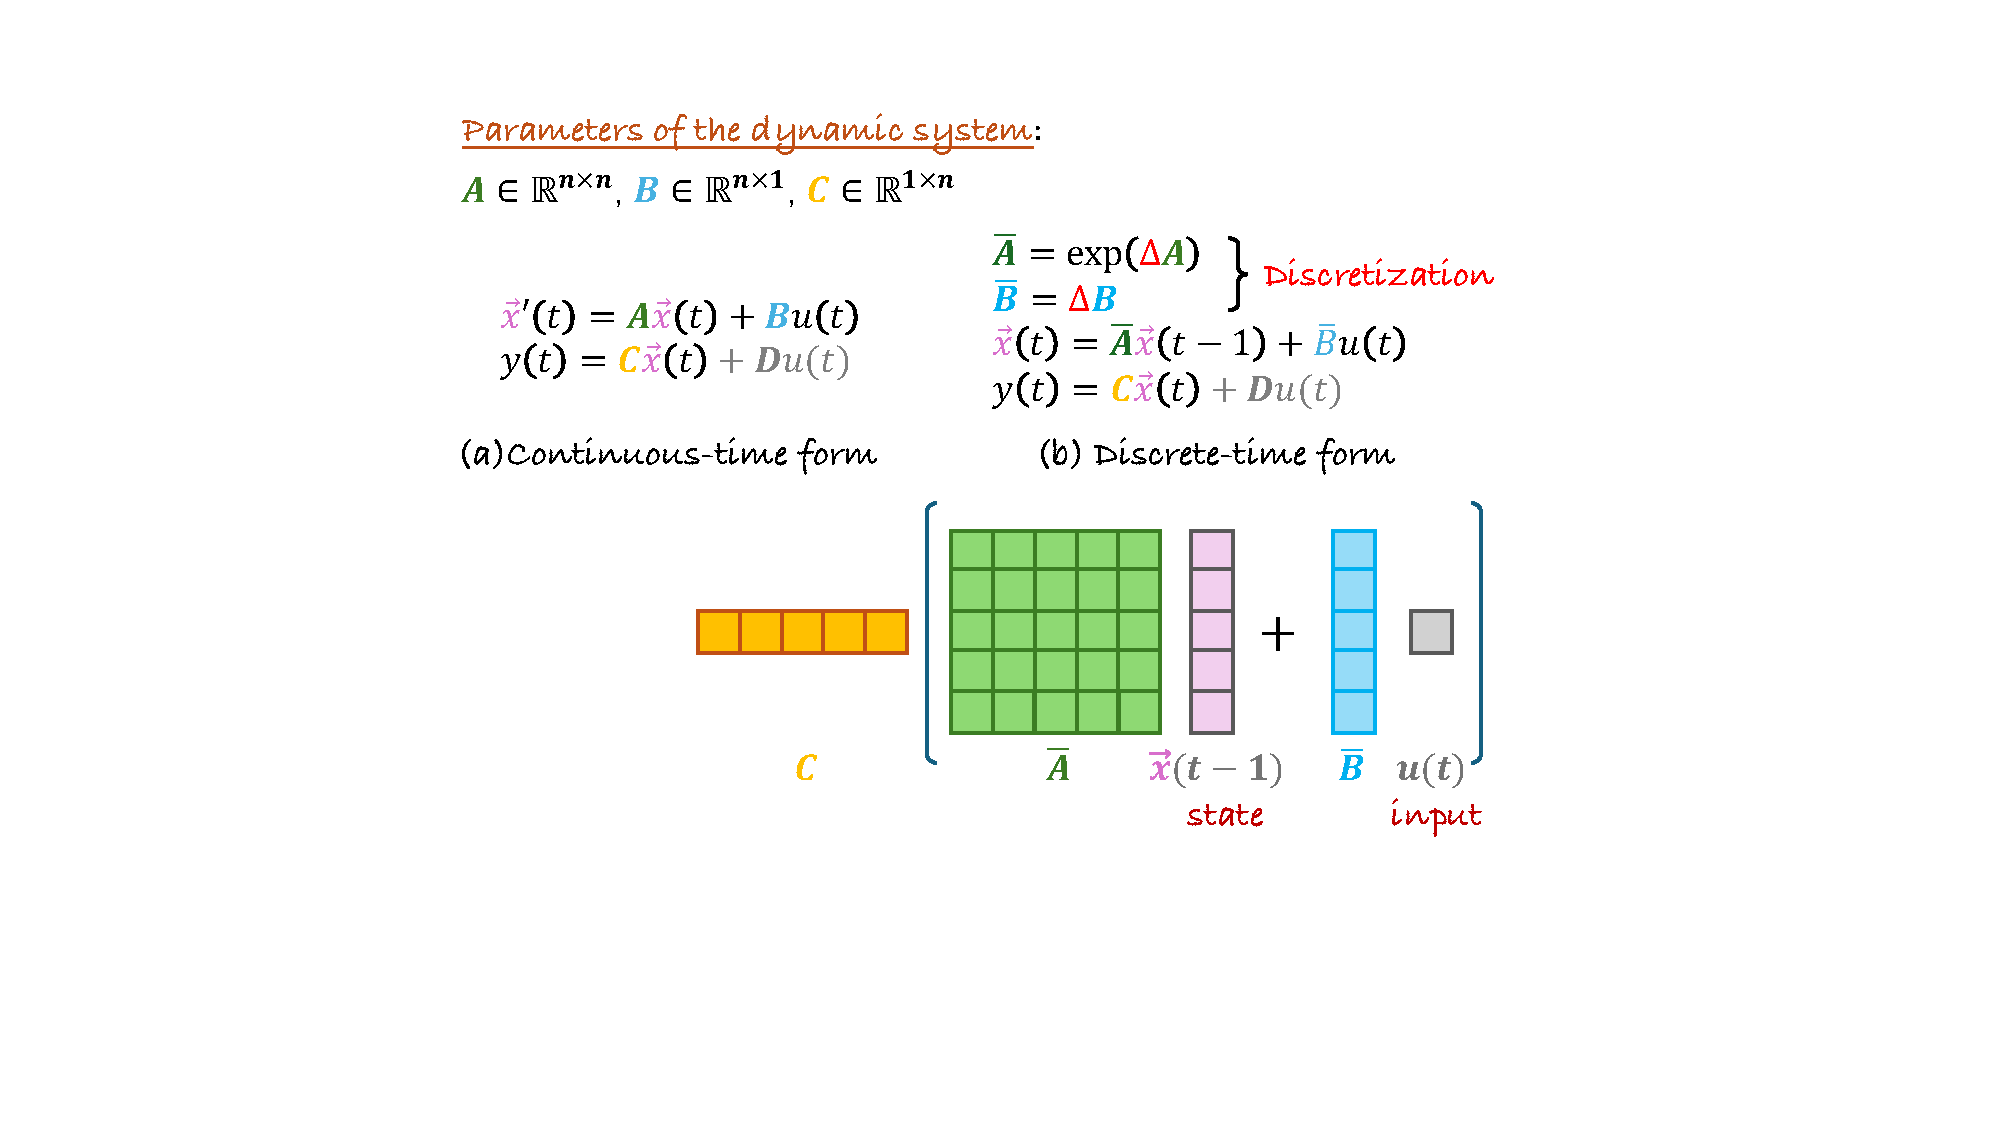
\includegraphics[width=0.6\textwidth]{figures/SSM-overview.pdf}
  \caption{作用于一个scalar input $u(t)$的SSM model,$\vec{x}$是状态}\label{fig:ssm-overview}
\end{figure}

机器学习任务中输入都是向量形式,假设为$D$。将图\ref{fig:ssm-overview}这样一个模型应用到向量输入的方法也非常直接:
引入$D$个独立的SSM模型,每个独立地作用于输入信号的一个维度。
假设输入序列的batch大小为:$B$,序列长度$L$,channel大小为$D$ (hidden size大小)。
于是,一个处理向量输入的SSM模型的有$DN$个参数。
处理完整个序列的时间和空间复杂度是:$O(BLDN)$,mamba的贡献之一是通过模型设计,解决这个时间和空间的复杂度。

% 使用data-dependent的gating进行decay,能够进一步改善学习效果。然后推导出这个gating机制的并行形式。

\newpage
\section{并行RNN}
\subsection{典型代表}

\subsubsection{RWKV\cite{peng2023rwkv}}

\subsubsection{LRU(Linear Recurrent Unit)\cite{orvieto2023resurrecting}}

\newpage
\section{General non-linear recurrence 的并行计算问题}
\subsection{SOAC: scan}

Second-order Array Combinator (SOAC):\textcolor{red}{\textit{\textbf{scan}}} 是所有的循环神经网络(recurrent neural networks)背后的核心并行pattern。接口和语义如下:

\begin{equation*}
    \begin{aligned}
        \textbf{scan} &::(\alpha, \beta \rightarrow \alpha) \rightarrow \alpha \rightarrow[\beta]^d_n \rightarrow [\alpha]_n^d \\
        \mathbf{scan} \ \oplus \ \textit{xs} &= [x_0,\ x_0 \oplus x_1, \dotsb,\ x_0 \oplus x_1 \dotsb \oplus x_n ] \\
        \mathbf{scanl} \ \oplus \ I \ \textit{xs} &= \left[
            I \oplus x_0,\  ((I \oplus x_0) \oplus x_1), \ \dotsb,
            \ (((I \oplus x_0)\oplus x_1)\dotsb \oplus x_{n-1})
        \right] \\
        \mathbf{scanr} \ \oplus \ I \ \textit{xs} &= \left[
            (x_0 \oplus (x_{n-2} \oplus (x_{n-1} \oplus I)))
            ,\ \dotsb, \ (x_{n-2} \oplus (x_{n-1} \oplus I)),
            \ x_{n-1} \oplus I \right] \\
    \end{aligned}
\end{equation*}


% If $\oplus$ is associative, scan can be executed in parallel\cite{DBLP:journals/tc/Blelloch89}.
% If $\oplus$ is left associative, scanl is used. If $\oplus$ is right associative, scanr is used. The first operand of $\oplus$ carries a data dependence with a distance of 1\cite{DBLP:journals/tpds/WolfL91}.

% \subsection{RNN}

% As shown in Figure \ref{scan-step}, in one computational step, a cell processing unit $\otimes$ produces a new token $y$ by aggregating a token $x$ from a token stream $xs$ with another token $y'$ created in the previous computational step.

% \begin{figure}[h]
%     \centering
%     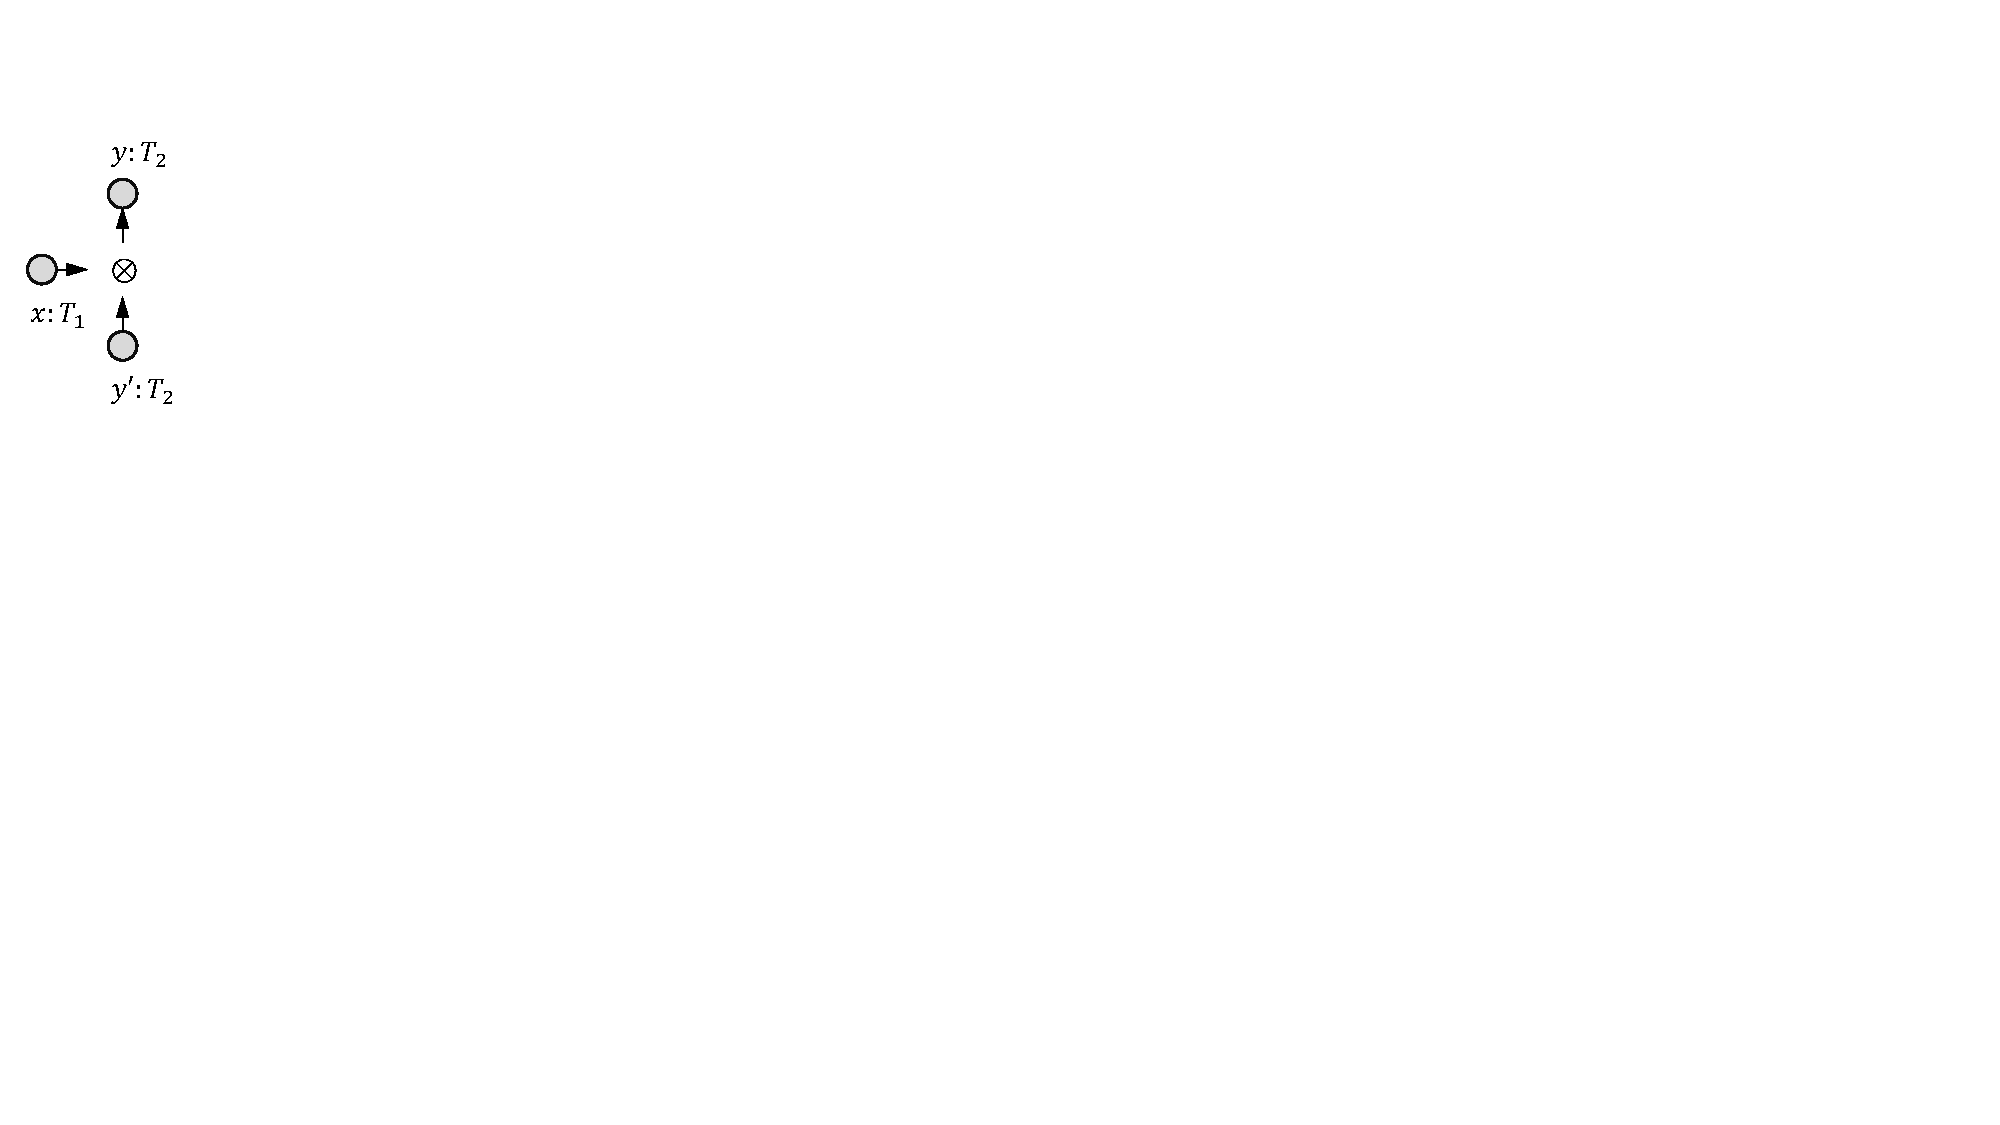
\includegraphics[width=0.1\textwidth]{figures/scan_step.pdf}
%     \caption{A single RNN computation step.}
%     \label{scan-step}
% \end{figure}

% Figure \ref{rnn-layer1} shows an algorithm developer's conceptual model of an RNN layer (the unrolled computational graph in mainstream deep learning frameworks) applied to tokens from a sequence.

% \begin{figure}[h]
%   \centering
%   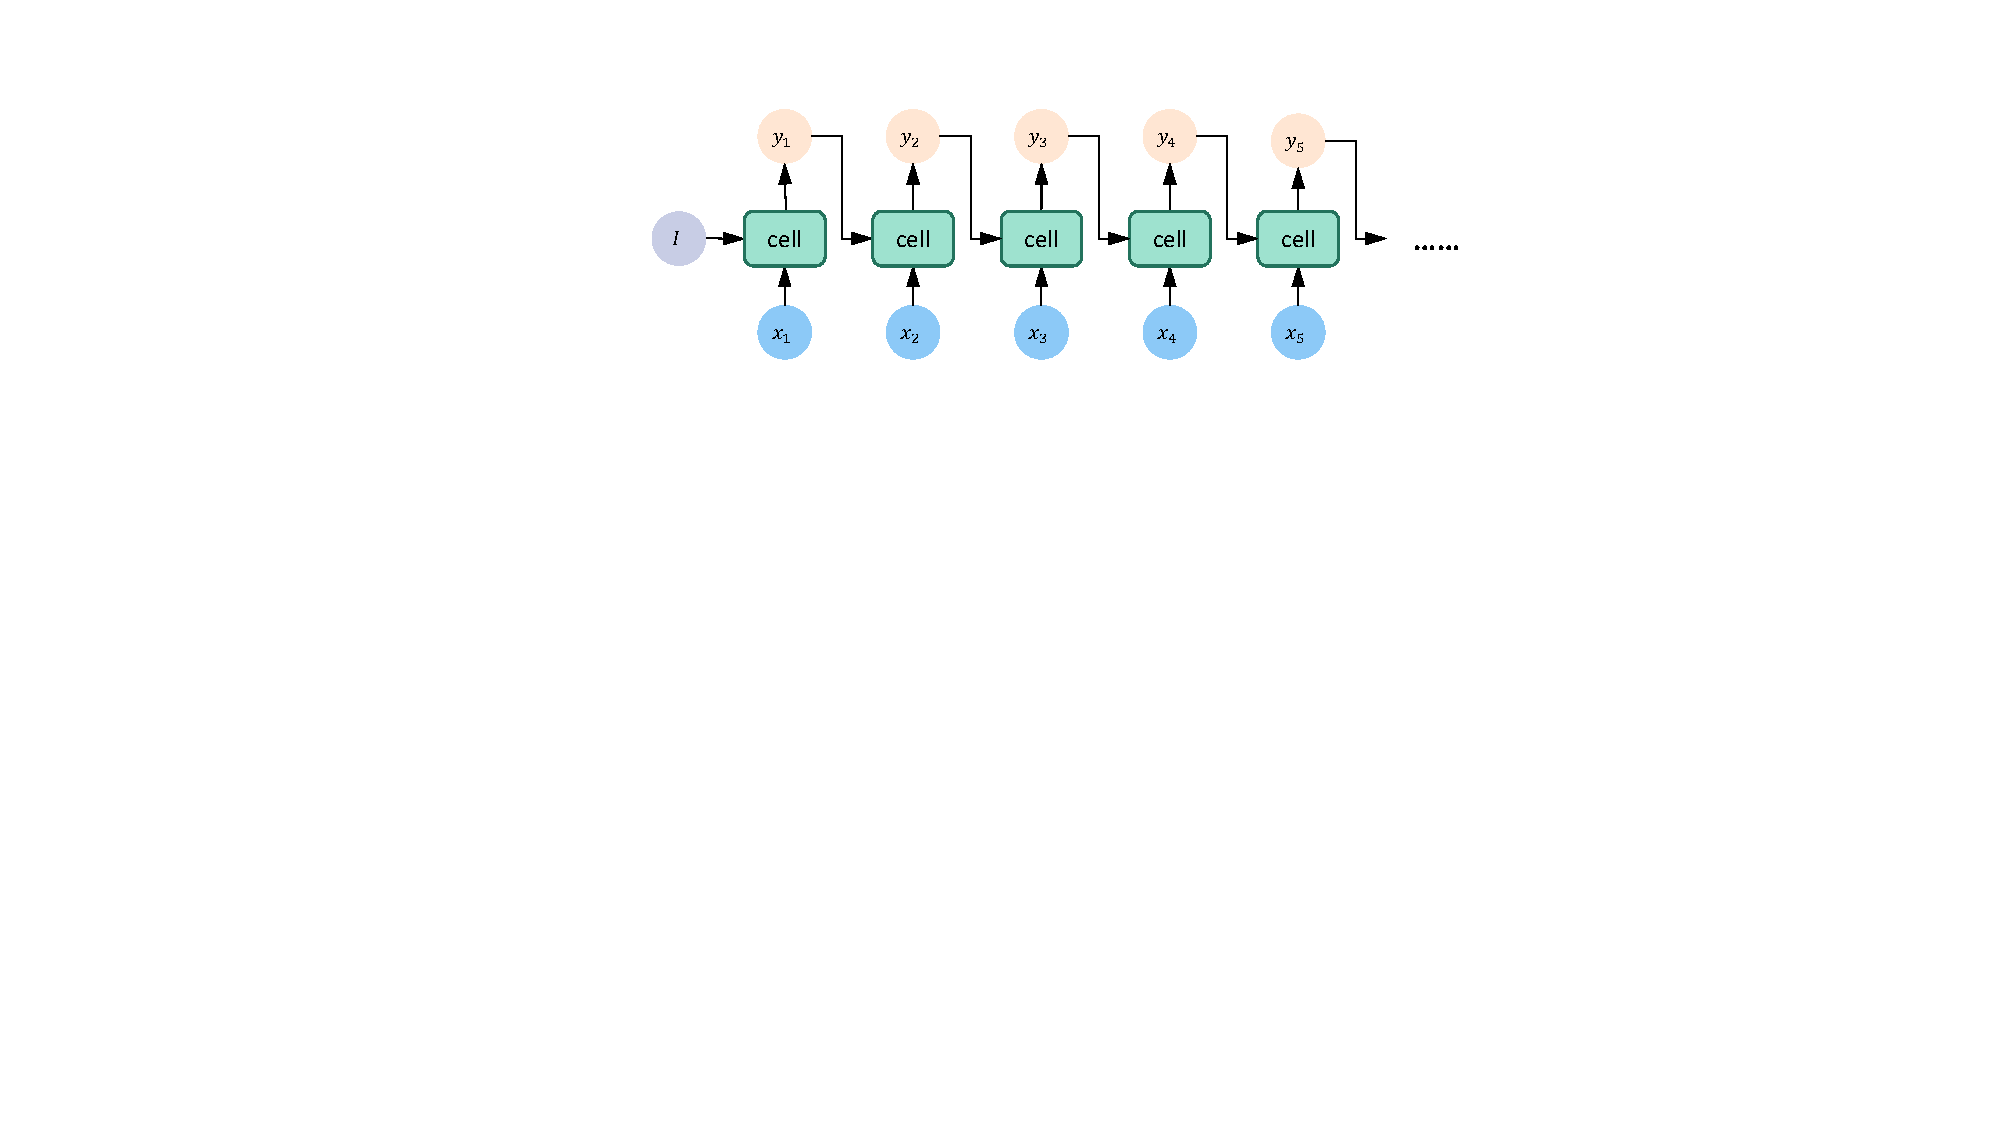
\includegraphics[width=0.5\textwidth]{figures/rnn_layer1.pdf}
%   \caption{An algorithm developer's conceptual model of an RNN layer applied to a single sequence.}
%   \label{rnn-layer1}
% \end{figure}

% An RNN layer is usually trained with a batch of sequences. Figure \ref{rnn-layer2} shows applies an RNN layer to multiple sequences simultaneously and Listing \ref{rnn-layer-code} is the corresponding codes using FractalTensor constructs.

% \begin{figure}[h]
%   \centering
%   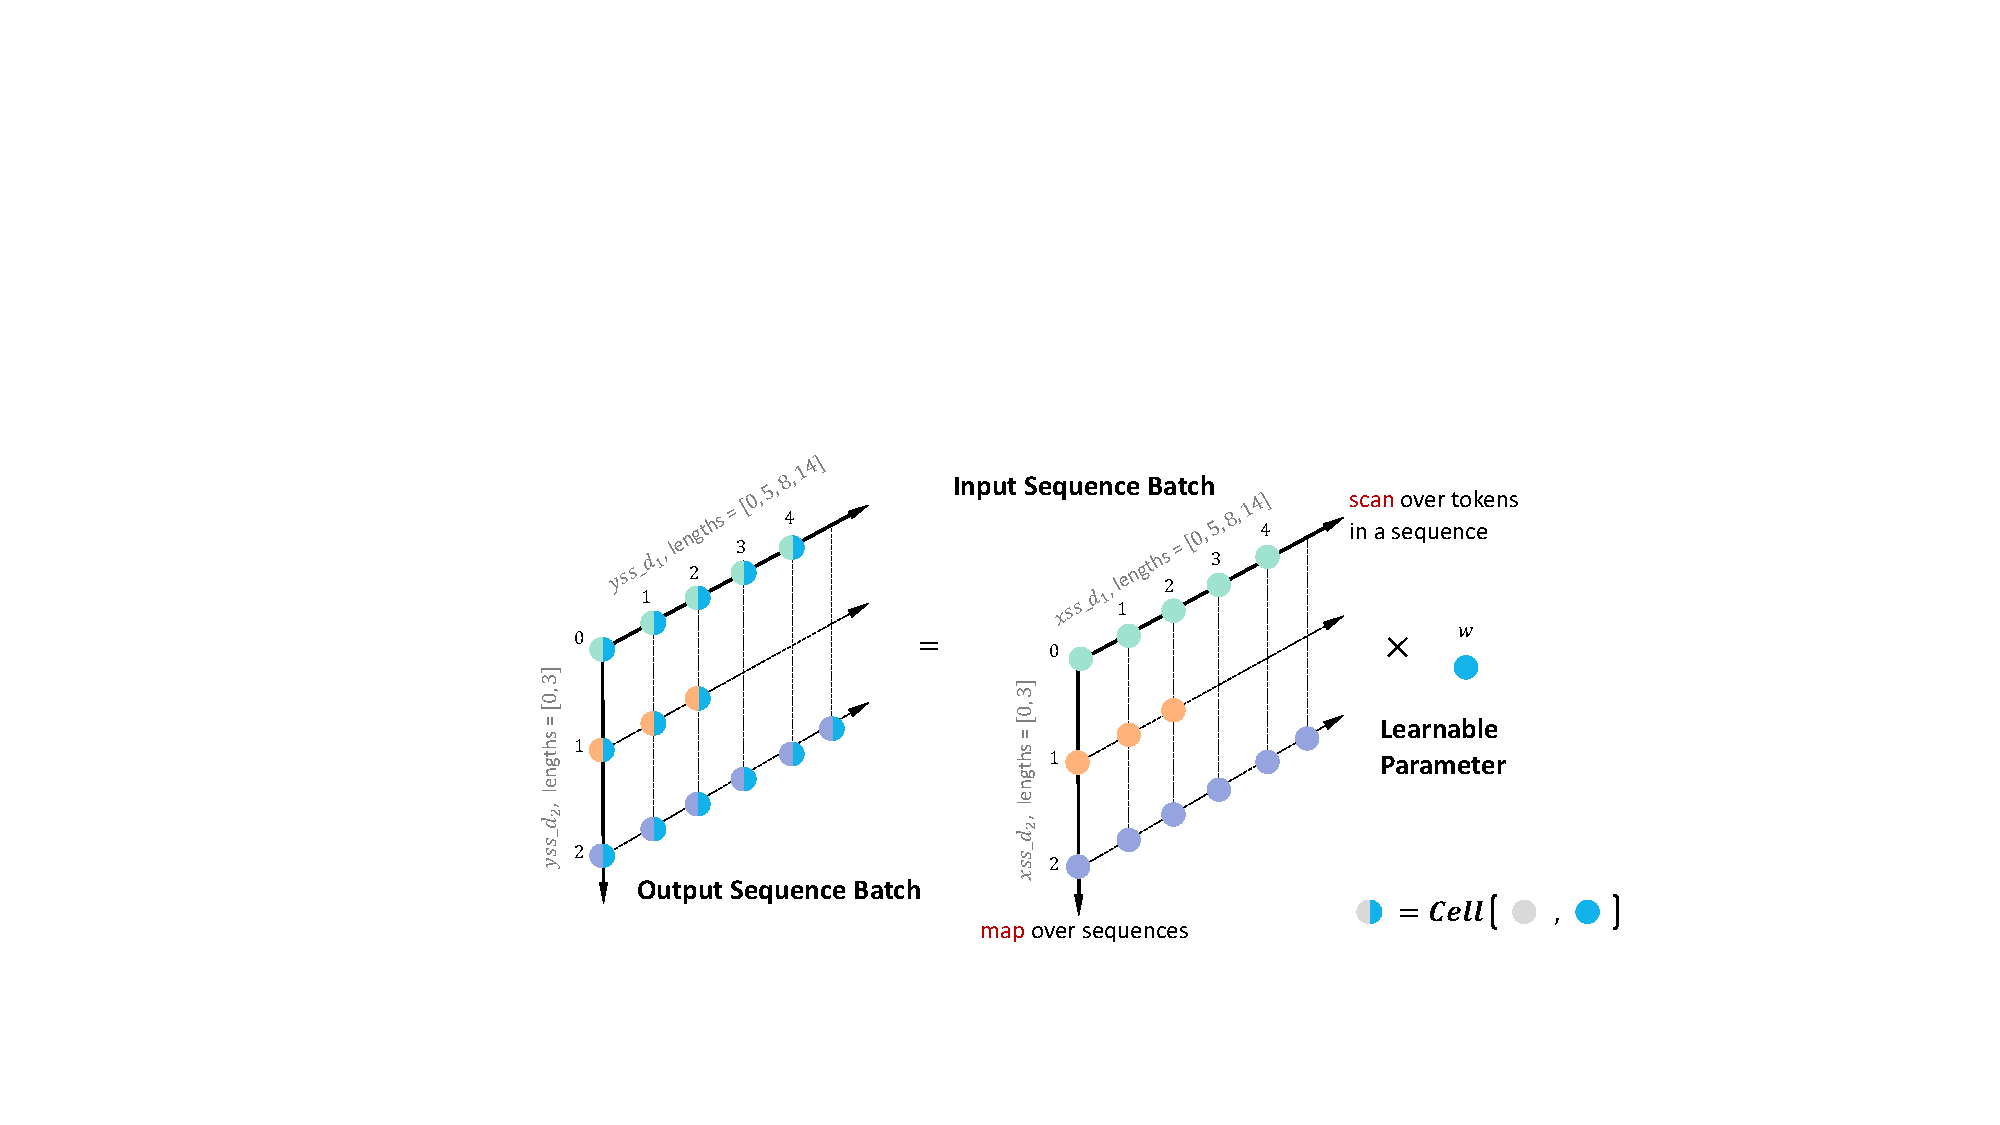
\includegraphics[width=0.6\textwidth]{figures/rnn_layer2.pdf}
%   \caption{An RNN layer applied to multiple sequences.}
%   \label{rnn-layer2}
% \end{figure}

% \lstset{
%   frame=lrtb,
%   backgroundcolor=\color{aliceblue},
%   numbers=left,
%   numbersep=5pt,
%   numbersep=1em,
%   xleftmargin=1em
% }
% \begin{lstlisting}[language=fractaltensor-hello-world, caption={用Parallel Pattern \textcolor{red}{\textit{map}}和\textcolor{red}{\textit{scan}}的嵌套compose 一个RNN layer}, label={rnn-layer-code}]
% xss: [][]float32[1, 512] = ...  // A batch of input sequences
% (:\textbf{\textcolor{dkgreen}{w}}:): float32[512, 512] = ...  // Learnable parameter for the UDF

% // yss: [][]float32[1, 512], the output buffer
% (:\textbf{\textcolor{dkgreen}{yss}}:) = xss.map(xs (:$\Rightarrow$:) {
%     ys = xs.scan(s, x (:$\Rightarrow$:) {
%         y = x @ (:\textbf{\textcolor{dkgreen}{w}}:) + s  // UDF is small math function
%     }, initializer=zeros),
% })
% \end{lstlisting}

% \begin{lstlisting}[language=cplus, caption={Listing \ref{rnn-layer-code}的imperative style 语法等价形}]
% xss: [][]float32[1, 512] = ...  // token batch
% (:\textbf{\textcolor{dkgreen}{w}}:): float32[512, 512] = ... // UDF的可学习参数
% yss: [][]float32[1, 512] = ... // 输出buffer

% L: const int[3] = [5, 3, 6]
% N: int = len(xss)

% for i = [0, N) {  // 对应了全并行的map
%   for j = [0, L[i]) {  // 对应了携带数据流依赖的scan
%     if j == 0:
%       s = zeros
%     else:
%       s = yss[i][j - 1]
%     x = xss[i][j]
    
%     yss[i][j] = x @ w + s
%   }
% }
% \end{lstlisting}


\newpage
\subsection{Stacked RNNs}

\begin{figure}[h]
  \centering
  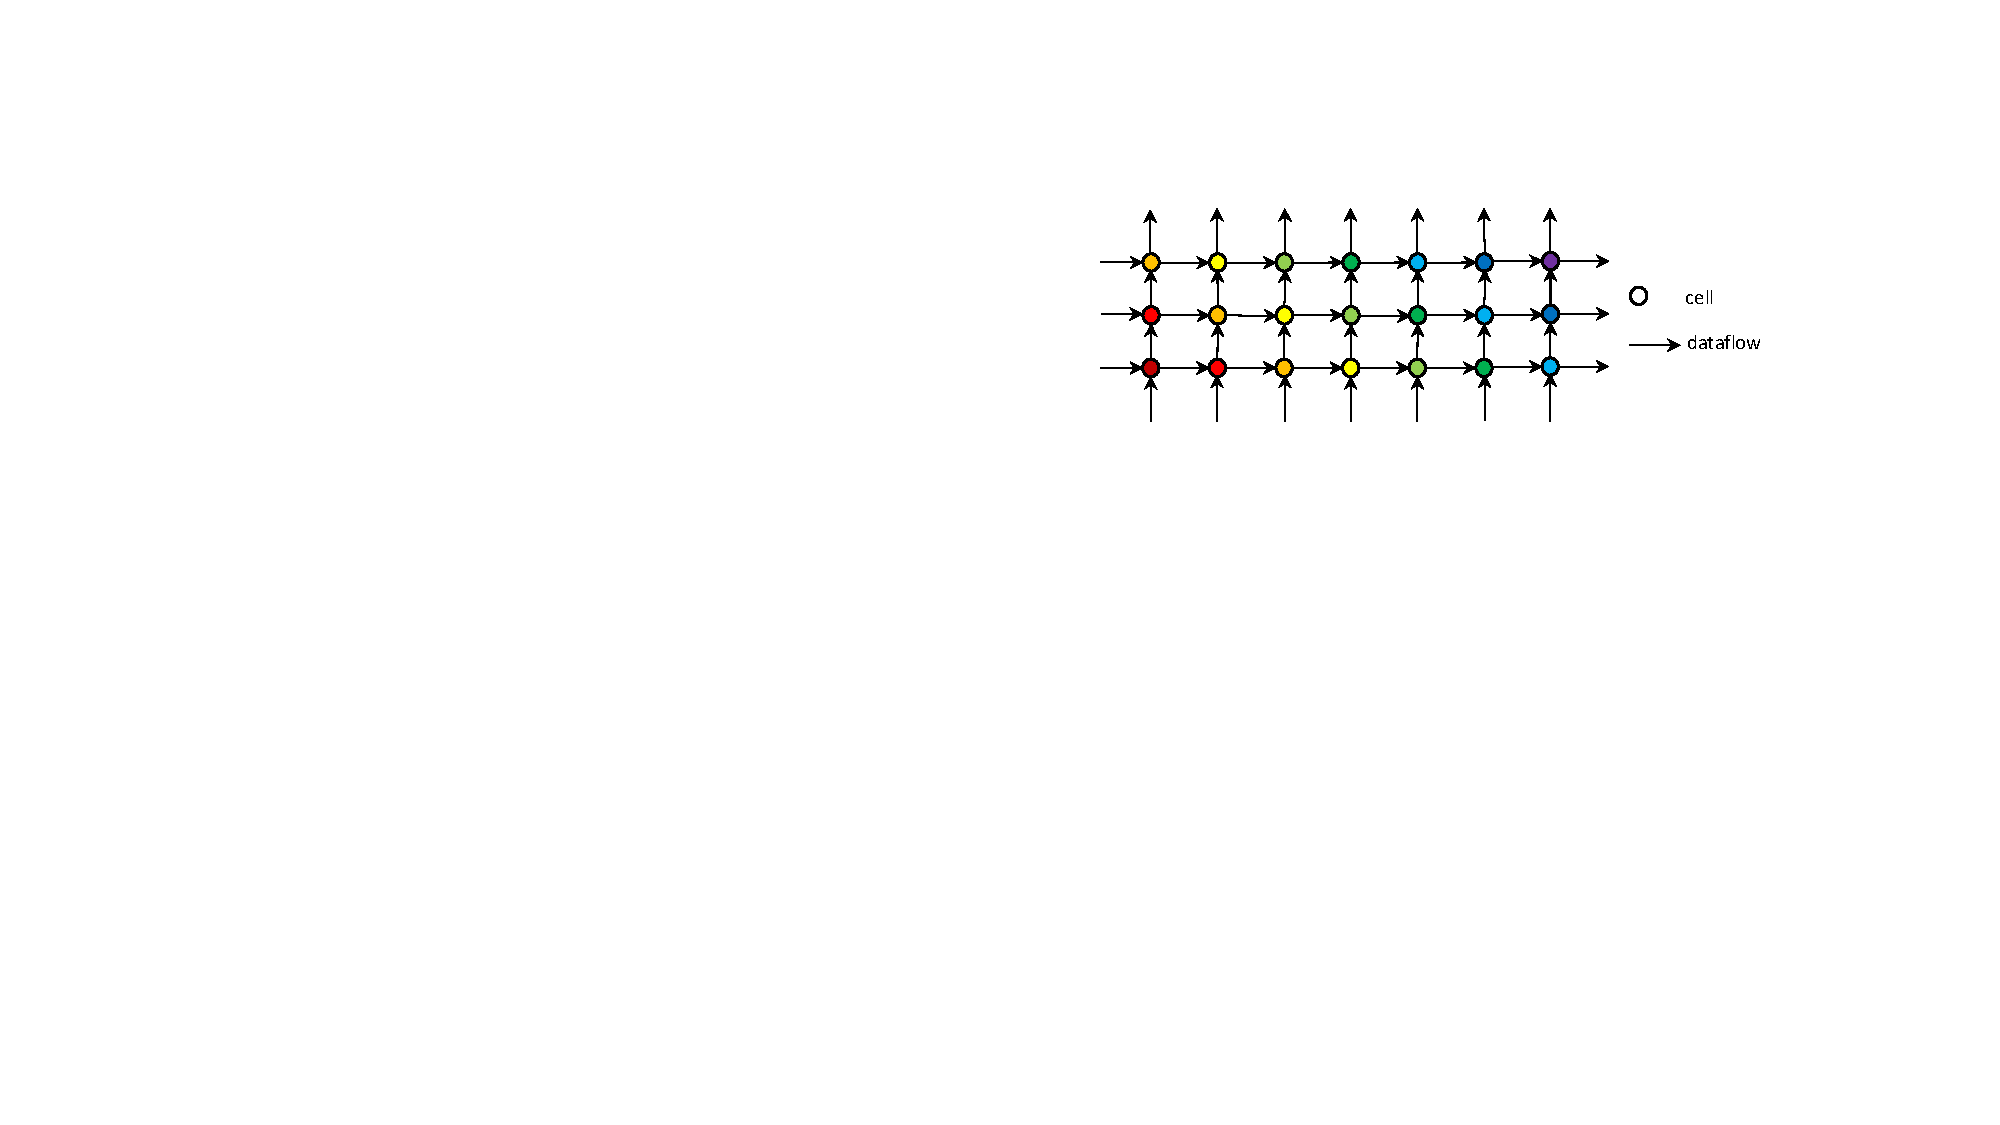
\includegraphics[width=0.6\textwidth]{figures/signal_flow_structure_of_stacked_rnn.pdf}
  \caption{Stacked RNN网络的数据流图}\label{fig:dataflow-stacked-rnn}
\end{figure}

一个optimizing compiler最关心的问题是:检测一个算法天生的\textcolor{blue}{最大并行性}和\textcolor{blue}{最大数据复用机会}。如果能检测到就有可能通过调度策略的设计,在一个并行后端上达到高效执行。
我们无论用什么样的语法形式去写RNN网络,对optimizing compiler检测和利用并行性最重要的是抽取出图\ref{fig:dataflow-stacked-rnn}这样的一个数据流图结构。
\vspace{1em}

\begin{lstlisting}[language=fractaltensor-hello-world, caption={用parallel pattern compose stacked RNN网络}, label={stacked-rnn-code1}]
xss: [][]float32[1, 512] = ...  // A batch of input sequences
ws: [3]float32[512, 512] = ...  // UDF的可学习参数

ysss = xss.map(xs => {  // ysss: [[[float32[1, 512]]]]
  yss = ws.scan(ss, w => {  // scan over depth
    ys = ss.scan(s, x => {  // scan over sequence length
      y = x @ w + s  // the user-defined cell function.
    }, initializer=zeros),
  }, initializer=xs),
})
\end{lstlisting}

\begin{lstlisting}[language=fractaltensor-hello-world, caption={Listing \ref{stacked-rnn-code1} 的另一种语法等价形}, label={stacked-rnn-code}]
xss: [][]float32[1, 512] = ...  // A batch of input sequences
ws: [3]float32[512, 512]] = ...  // UDF的可学习参数

ysss = xss.map(xs => {  // ysss: [][][]float32[1, 512]
  yss = xs.scan(ss, x => {  // scan over sequence length
    ys = zip(ss, ws).scan(s0, s, w => { // scan over depth
      y = s0 @ w + s  // UDF是一个非常小的纯线性代数公式
    }, initializer=x),
  }, initializer=repeat(zeros, ws.length)),
})
\end{lstlisting}

这里有一个非常漂亮的特性,对并行性检测和利用至关重要,\textit{\textbf{\textcolor{red}{用map,reduce,scan 这样的SOAC写出来的嵌套循环程序,一定是一个可任意换序的循环嵌套}}}。

\newpage
\begin{lstlisting}[language=cplus, caption={Stacked RNN的imperative style语法等价形,这里把UDF替换成LSTM的cell function}, label={stacked-lstm-imperative}]
for i in range(N):  // corresponds to map
  for j in range(D):  // corresponds to fold
    for k in range(L):  // corresponds to scan
      if j == 0 and k == 0: // control region S0
        h_prev = zeros
        c_prev = zeros
        x = xss[i][k]
      elif j == 0 and k > 0: // control region S1
        h_prev = hsss[i][j][k - 1]
        c_prev = csss[i][j][k - 1]
        x = xss[i][k]
      elif j > 0 and k == 0: // control region S2
        h_prev = zeros
        c_prev = zeros
        x = hsss[i][j - 1][k]
      else:  // control region S3
        h_prev = output[i][j][k - 1]
        c_prev = output[i][j][k - 1]
        x = hsss[i][j - 1][k]
  
      h, c = lstm_cells[j](x, h_prev, c_prev) // the UDF
      hsss[i][j][k] = h
      csss[i][j][k] = c
\end{lstlisting}

Listing \ref{stacked-lstm-imperative} 是stacked RNN网络的语法等价形式,唯一变化是这里我们把UDF替换成LSTM cell:
$c_t, h_t = \textbf{lstm\_cell}\left(\vec{x}_t,\vec{h}_{t-1}, \mathbf{Params} \right)$,具体是由下面六个线性代数公式定义:

\begin{align}
     f_t &= \sigma_g\left(\mathbf{W}_f\vec{x}_t + \mathbf{U}_f \vec{h}_{t-1}+\vec{b}_f\right) \\
     i_t &= \sigma_g\left(\mathbf{W}_i\vec{x}_t + \mathbf{U}_i \vec{h}_{t-1}+\vec{b}_i\right) \\
     o_t &= \sigma_g\left(\mathbf{W}_o\vec{x}_t + \mathbf{U}_o \vec{h}_{t-1}+\vec{b}_o\right) \\
     \widetilde{c}_t &= \sigma_c\left(\mathbf{W}_c\vec{x}_t + \mathbf{U}_c \vec{h}_{t-1}+\vec{b}_c\right) \\
     c_t &= f_t \odot c_{t-1} + i_t \odot \widetilde{c}_t \\
     h_t & = o_t \odot \sigma_h\left(c_t\right)
\end{align}

于是,我们会面对这样一个问题:\textit{\textbf{\textcolor{tomato}{给定了这样一组嵌套在loop nest之中的线性代数公式:LSTM cell,是否有办法让一个optimzing compiler基于程序中的general facts,同时给定硬件参数,自动推断出一个好的并行实现方案?}}} (我们的思考甚至\textit{可以安全地忽略}这个loop nest到底是用哪一种语法形式写出来的)。

\begin{figure}[h]
  \centering
  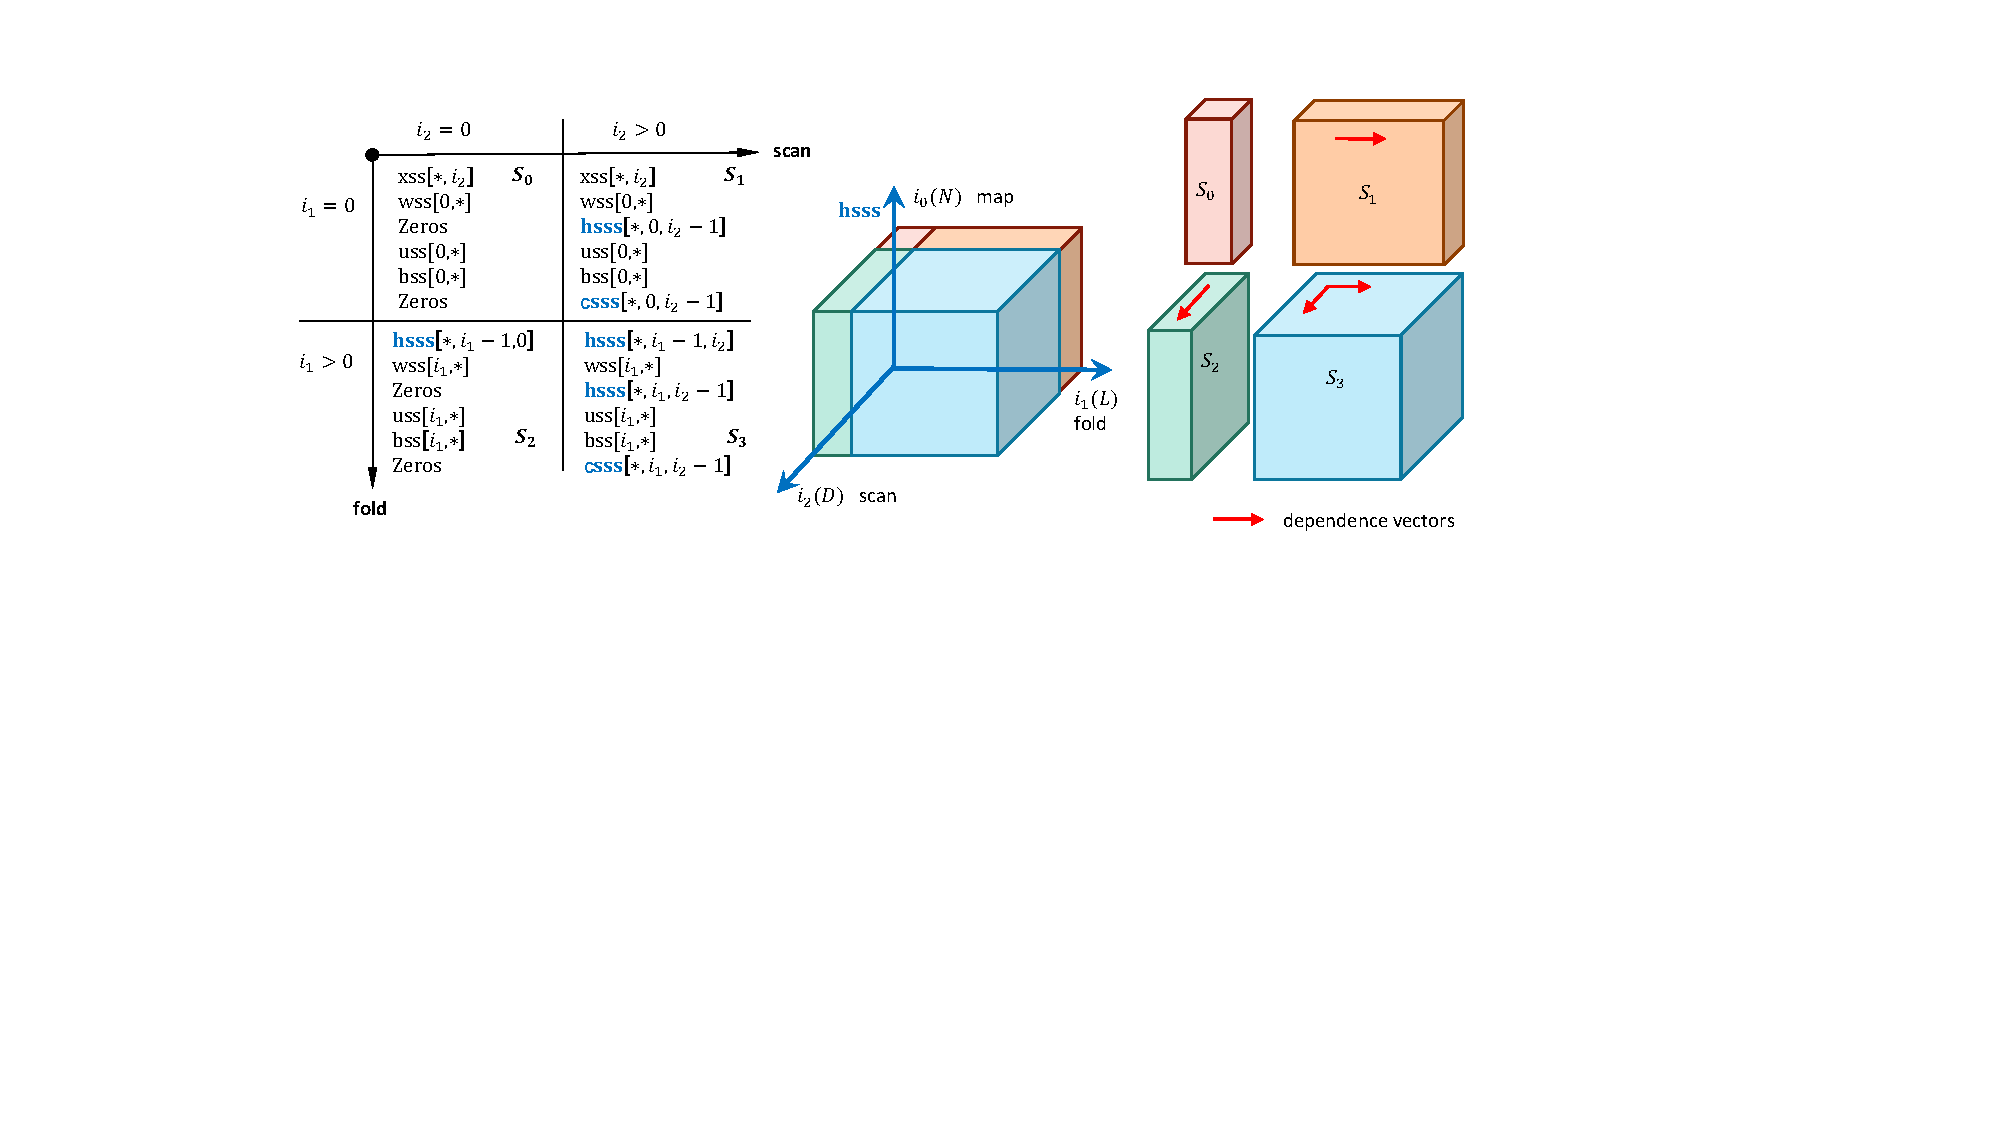
\includegraphics[width=1.\textwidth]{figures/cond_branchs.pdf}
  \caption{编译stacked RNNs计算的复杂性}\label{cond_branchs}
\end{figure}
\subsection{循环倾斜后循环边界的上下界的求解}

约定loop nest深度的计数从循环最外层向循环体递减,也就是最外层层数最深,循环体深度记为$d = 0$。

图\ref{cond_branchs}中数据流依赖最复杂的控制区域$s_3$用等价的imperative for loop写出来如下:
\begin{lstlisting}[language=cplus]
for (:$i$:) in range (:$[0, N)$:):  // map, 全并行
  for (:$j$:) in range (:$[1, D)$:):  // scan,控制深度2携带数据流依赖
    for (:$k$:) in range (:$1, L)$:):  // scan,控制深度1携带数据流依赖
        (:\textit{UDF}:)(...)
\end{lstlisting}

以上嵌套循环程序的迭代空间是一个三维立方体,可以用如下不等式表示:

\begin{equation}
\begin{aligned}
0 &\le i < N \\
1 &\le j < D \\
1 &\le k < L
\end{aligned}\label{eq:bounds}
\end{equation}

如果我们把迭代空间看做是一个三维空间中的整数点集合,整个循环体看做一个statement,记作$s_x$。x是迭代空间中的一个整数点,也就是$s$的一次执行。
$s_{i_1, j_1, k_1}$写,$s_{i_2, j_2, k_2}$读同一个buffer位置,这两次执行之间存在数据流依赖。
图\ref{fig:dataflow-stacked-rnn}直观地揭示了另一个关于计算过程数据流依赖情况的事实:上面这个loop nest在迭代空间中携带了\textbf{\textcolor{blue}{两类}}数据流,读和写之间的距离是:
$d_1 = [0, 1, 0]$和$d_2 = [0, 0, 1]$。
loop nest中的数据流依赖可以用如下dependence distance vector矩阵$M$描述:

\begin{equation*}
    \begin{bmatrix}
        \vec{d_1} & \vec{d_2}
    \end{bmatrix} = 
    \begin{bmatrix}
        0 & 0 \\ 1 & 0 \\ 0 & 1
    \end{bmatrix}
\end{equation*}

我们要求解的一个调度问题是,给定$M$作为约束,求解一个变化矩阵$T$,能够让最外层循环携带所有数据流依赖。
这里我们暂时忽略矩阵$T$是如何得到的,只需要先记住$T$不唯一,$T$的求解是一个well-studied问题,有完善的理论和工具。
下面直接给出$T$的一种可能结果:

\begin{equation*}
    \delta_A =
    \begin{bmatrix}
        0 & 1 & 1 \\ 1 & 0 & 0 \\ 0 & 1 & 0
    \end{bmatrix}
    \begin{bmatrix}
        i \\ j \\ k
    \end{bmatrix} =
    \begin{bmatrix}
        j+k \\ i \\ j
    \end{bmatrix} =
    \begin{bmatrix}
        m \\ n \\ p
    \end{bmatrix}
\end{equation*}

于是有:
\begin{equation}
    \begin{bmatrix}
        i \\ j \\ k
    \end{bmatrix} =
    \begin{bmatrix}
        n \\ p \\ m-p
    \end{bmatrix}\label{eq:skew}
\end{equation}

我们会得以$m$, $n$, $p$为迭代变量的变化后的循环程序。循环体执行时,在遇到$i$,$j$,$k$的地方,带入\eqref{eq:skew}。
那么下一个问题是,变化后的循环边界如何求解?(\textcolor{brown}{Fourier-Motzkin Elimination算法就是专门解决这个问题的方法}。isl这样的polyhedral工具都集成了这一算法)

\begin{lstlisting}[language=cplus]
for (:$m$:) in range (:$\textcolor{red}{?}$:):  // map, 全并行
  for (:$n$:) in range (:$\textcolor{red}{?}$:):  // scan,控制深度2携带数据流依赖
    for (:$p$:) in range (:$\textcolor{red}{?}$:):  // scan,控制深度1携带数据流依赖
        (:\textit{UDF}:)(...)
\end{lstlisting}

这里我们手算一下变化后的循环边界。

把\eqref{eq:skew}带入\eqref{eq:bounds}我们会得到:

\begin{align}
\textcolor{dkgreen}{0} &\textcolor{dkgreen}{\le n < N} \\
1 &\le p < D  \label{eq:bound-d}\\
1 &\le m - p < L \label{eq:bound-l}
\end{align}

最外层的循环边界必须是常数。将\eqref{eq:bound-d}和\eqref{eq:bound-l}相加我们能够得到最外层的循环边界:
\textcolor{dkgreen}{$$2 \le m < L + D -1$$}

从\eqref{eq:bound-l}我们能得到:$m - L < p \le m -1$,即:$m -L+1 \le p < m$;同时,$p$必须满足\eqref{eq:bound-d}的约束。这两个不等式求交集就是$p$的上下界:
\textcolor{dkgreen}{$$\text{max}(1, m -L+1) \le p < \text{min}(m, D)$$}

\textcolor{dkgreen}{绿色}标注的三个不等式就是变换后循环的上下界,我们会得到下面这样一个变化后的程序:
\begin{lstlisting}[language=cplus]
for (:$m$:) in range (:$[2, L + D - 1)$:)  // 串行
  {  // 把所有可并行的数据batch成一个更大的数据,插入对gather_nd的调用
    for (:$n$:) in range (:$[0, N)$:)  // 并行
      for (:$p$:) in range (:[$\max(1, m - L + 1),\ \ \min(m, D))$:) // 并行
          batched_data = gather(可并行的数据点)
  }
  UDF(batched_data)
\end{lstlisting}


\begin{appendices}
若存在可逆矩阵$P$,使得一个关于矩阵$A$的如下等式成立:
$$A = (PDP)^{-1}$$

则称符合这样关系的矩阵$A$与$D$是相似矩阵,记作:$A \sim D$,则$A$的幂可以通过求矩阵$D$的幂求得

$$A^{m} = (PDP^{-1})^{m} = (PDP^{-1})(PDP^{-1})\dots(PDP^{-1})=PD^{m}P$$

\textcolor{red}{如果我们能够得出$D$是一个很简单的矩阵,例如对角矩阵,那么就可以很简单的计算出$A$的幂值}。
然而,一般的矩阵在实数域不一定能对角化,然而几乎所有矩阵都能在复数域对角化\cite{lru-kexue}。
于是$A$总能写成:

\begin{align*}
A=P\Lambda P^{-1} & A^{m} = P\Lambda^{m} P^{-1}
\end{align*}
\end{appendices}

\newpage
\bibliography{references.bib}
\end{document}
